\chapter{Réalisation de l'application}
\minitoc
\clearpage
\section{Introduction} Dans ce chapitre, on décrira toutes les fonctionnalités de l'application, leurs fonctionnement, les différents scénarii d'exécution avec des captures d'écran de chaque interface d'utilisateur avec un diagramme de séquences qui décrit en détail la fonctionnalité mentionnée
\justifying
\section{Création de compte}
La première étape pour utiliser l'application SPN-Cars est de créer un compte. Ce compte permettra aux utilisateurs de bénéficier de tous les services offerts par l'application.\\
\noindent Pour créer un compte, l'utilisateur a la possibilité de choisir trois méthodes : Créer un compte avec son émail et choisir un mot de passe, ou créer un compte tout simplement en utilisant l'option de création de compte avec son compte Google ou Apple.
\subsection{Création de compte avec email et mot de passe}
C'est la méthode la plus basique qui existe depuis toujours. Pour créer un compte, l'utilisateur doit tout d'abord entrer son adresse email, un mot de passe, et une confirmation de ce mot de passe. Lors de l'appui sur le bouton de <<Créer un compte>>, l'application envoie une requête vers le serveur back-end afin de vérifier l'existence d'un compte d'utilisateur utilisant la même adresse e-mail. Après une recherche effectuée sur les utilisateurs, le serveur back-end envoie une réponse positive s'il n'a trouvé aucun compte d'utilisateur utilisant l'adresse e-mail entrée par l'utilisateur, sinon une réponse négative sera envoyée. Selon la réponse retournée par le serveur l'application redirigera l'utilisateur vers une page pour compléter l'étape de création de compte si la réponse du serveur est positive, ou affiche un message d'erreur avec l'erreur adéquate si la réponse du serveur est négative.
\newpage
\begin{multicols}{2}
    \begin{figure}[H]
        \begin{center}
            \centering
            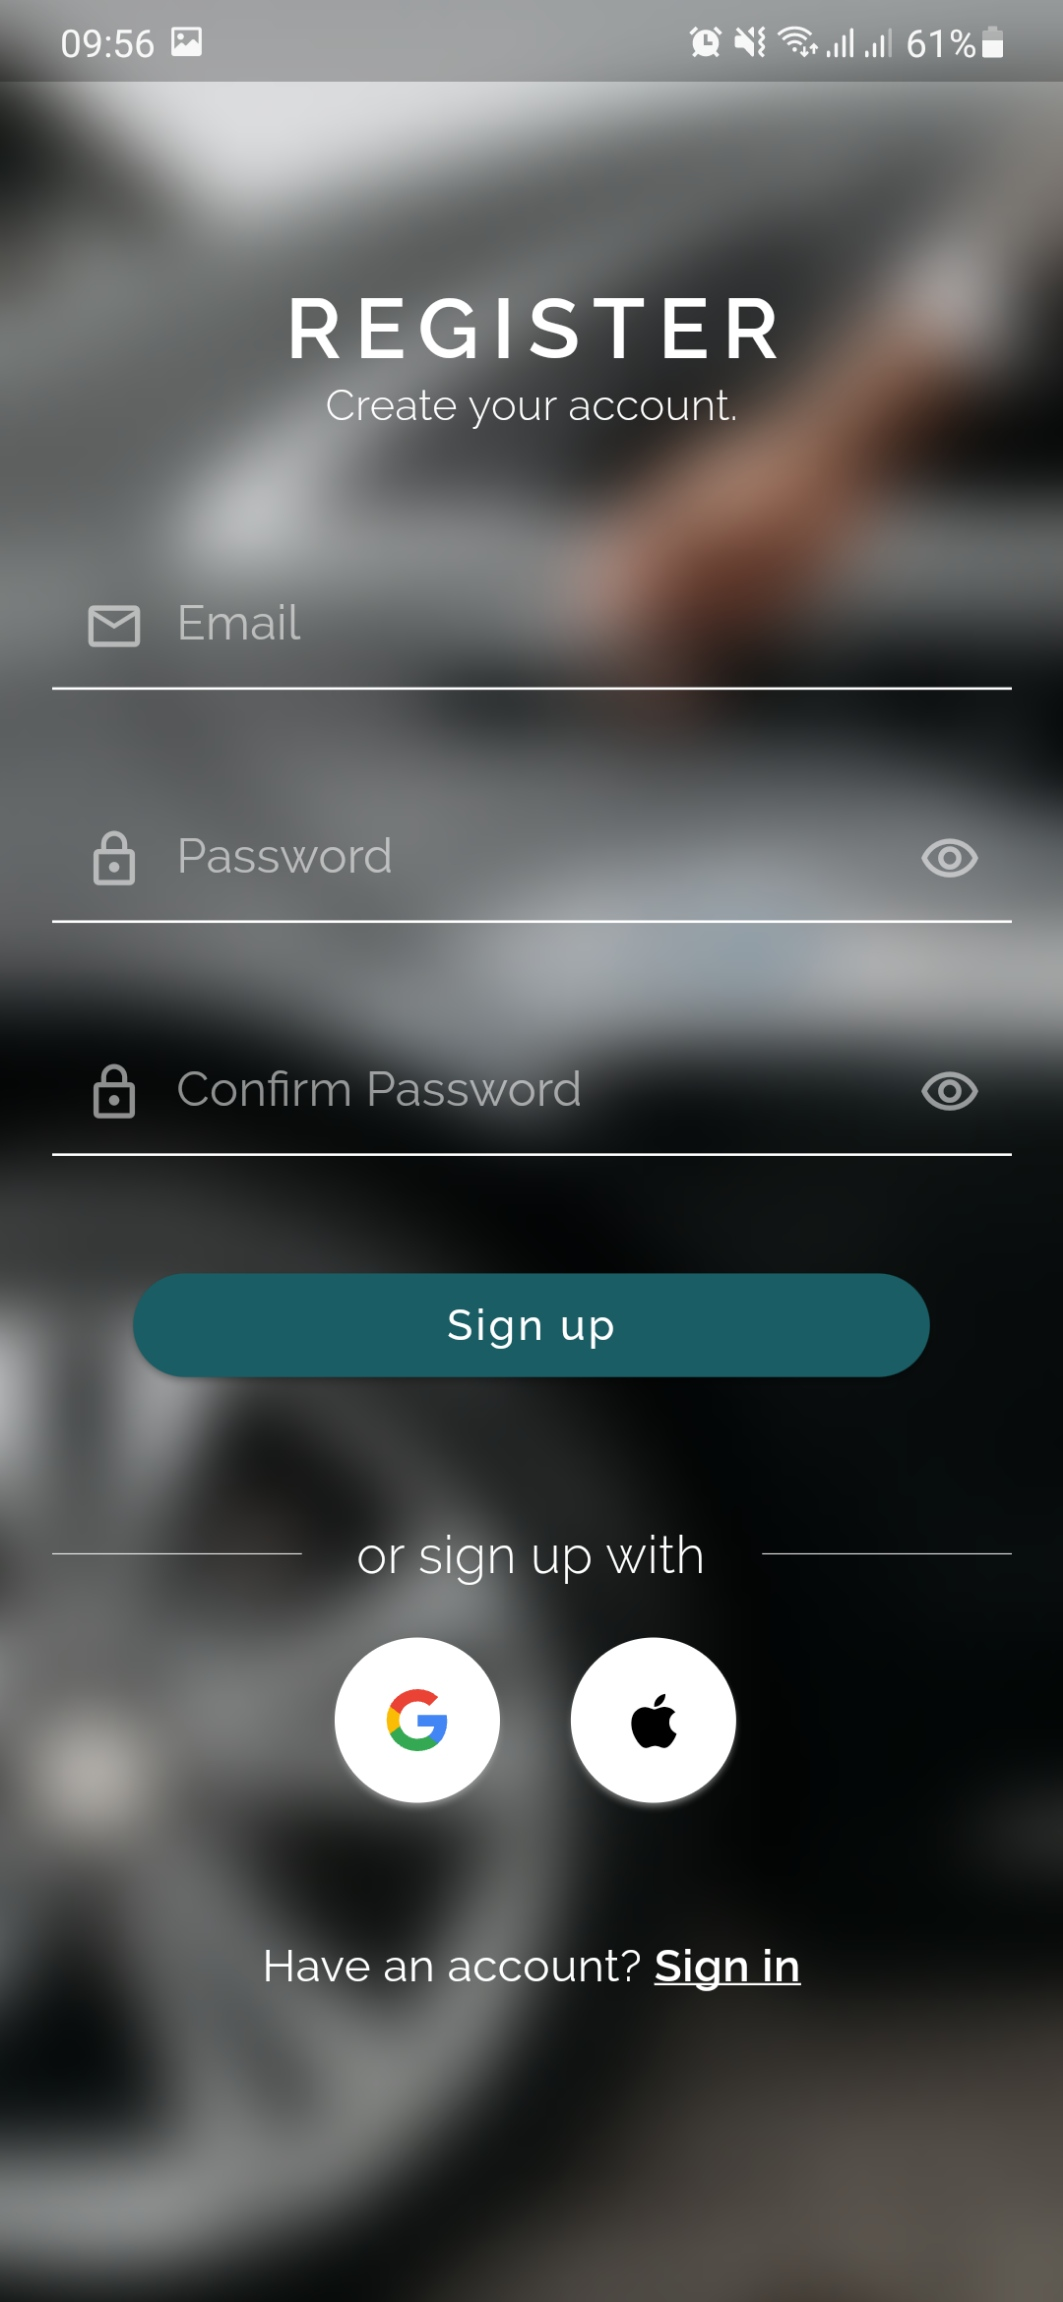
\includegraphics[height = 0.4 \textheight]{ui_screenshots/app_screenshots/register.png}
            \captionsetup{justification=centering}
            \caption{Formulaire de création de compte : 1ère étape.}
            \label{fig:app_register}
        \end{center}
    \end{figure}
    \begin{figure}[H]
        \begin{center}
            \centering
            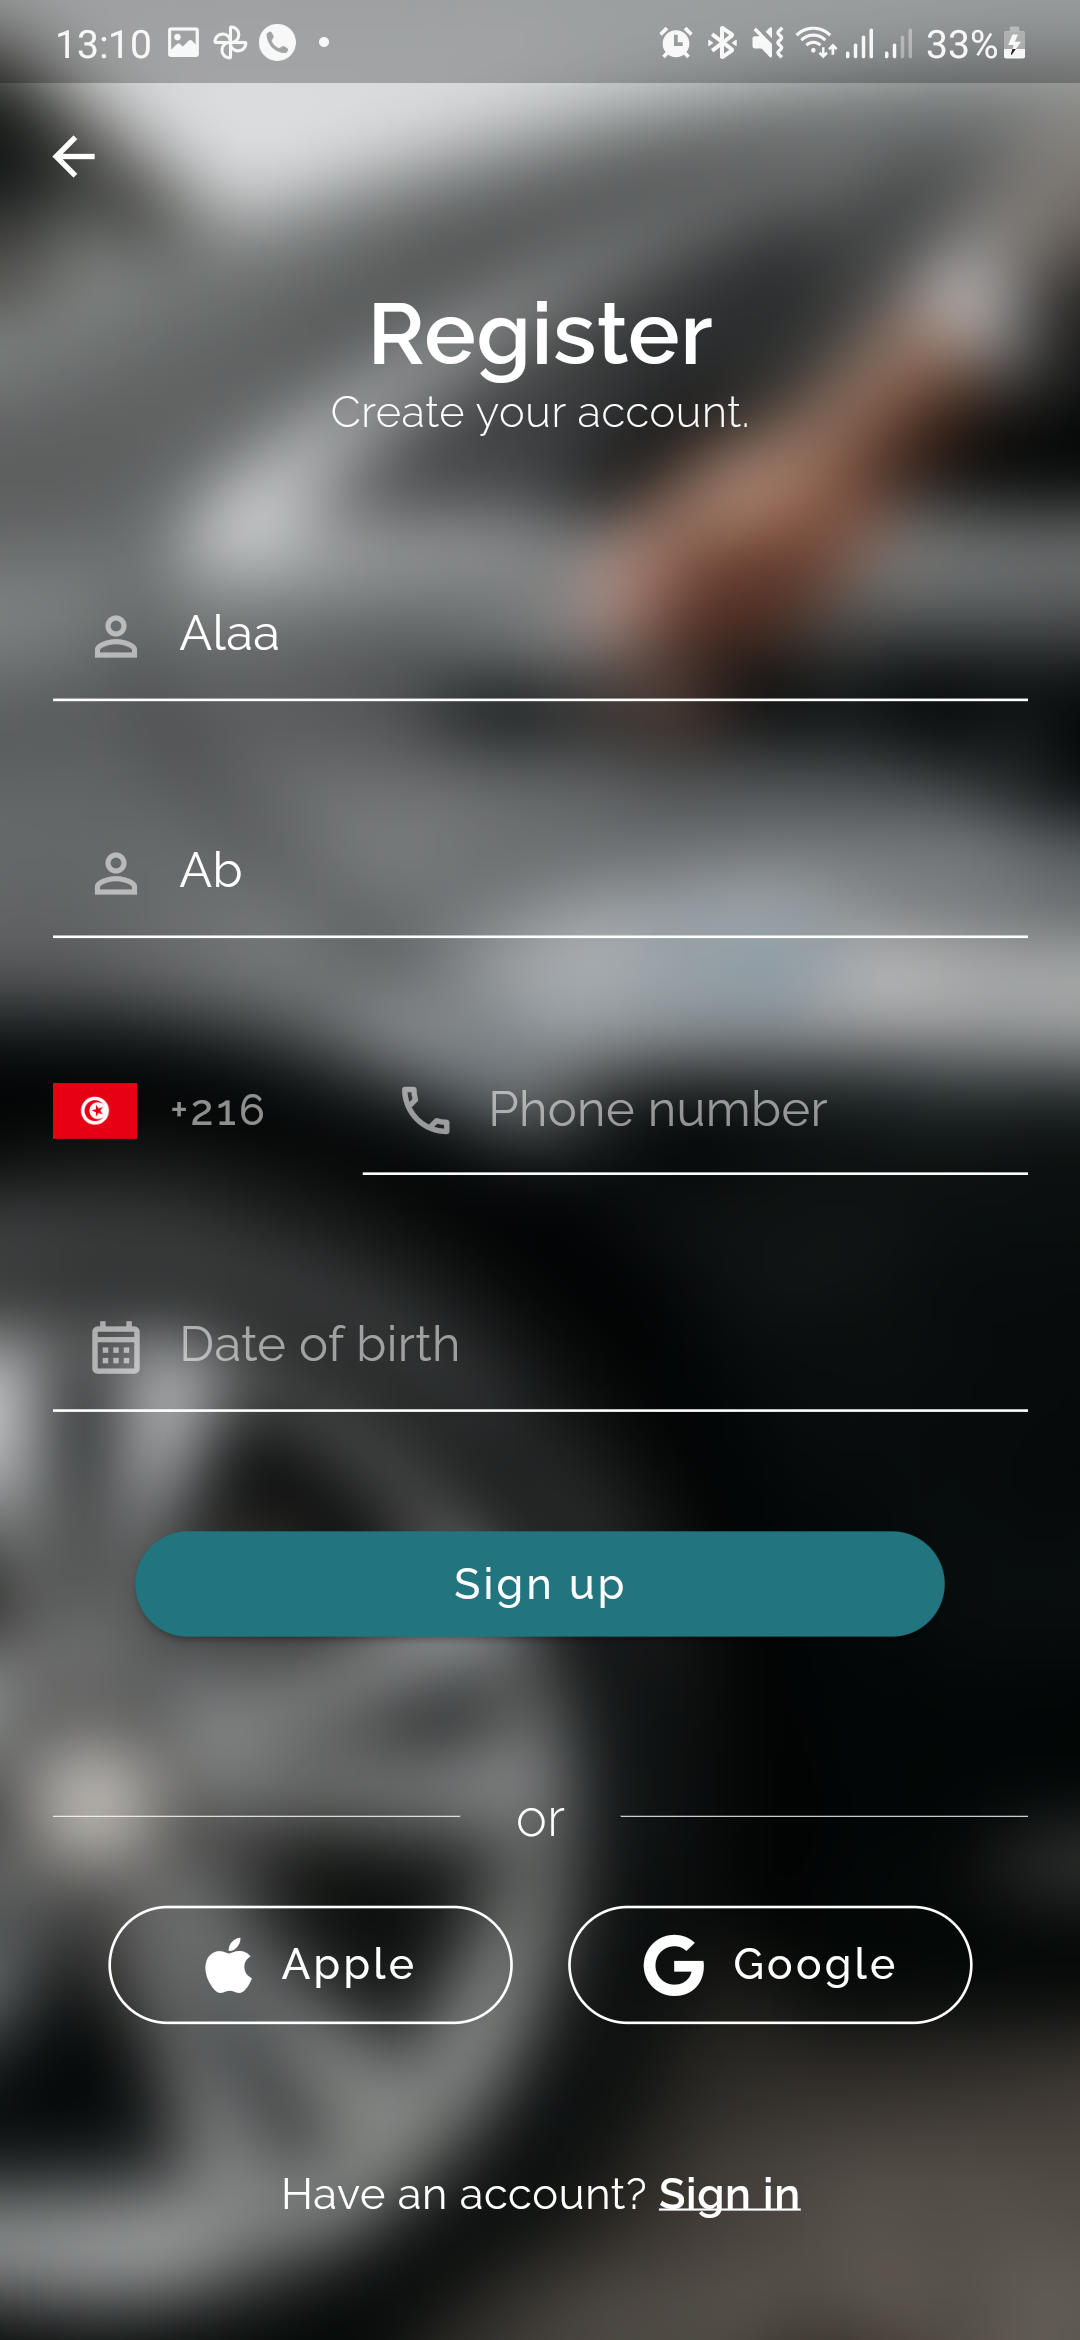
\includegraphics[height = 0.4 \textheight]{ui_screenshots/app_screenshots/finsih_register.png}
            \captionsetup{justification=centering}
            \caption{Formulaire de création de compte : 2ème étape.}
            \label{fig:app_finish_register}
        \end{center}
    \end{figure}
\end{multicols}
\subsection{Création de compte avec Google ou Apple}
Cette méthode est la plus facile et la plus rapide pour créer un compte ou s'authentifier. Avec un simple appui sur le bouton adéquat, une requête envoyée aux services de Google ou Apple pour récupérer les données du compte choisi. Ses données sont :
\begin{itemize}
    \item Un identifiant unique du compte Google ou Apple.
    \item L'adresse email du compte.
    \item Le nom et prénom utilisés avec le compte.
    \item La photo de profil utilisée avec ce compte.
\end{itemize}
Ses informations seront nécessaires pour passer la première étape de création de compte et avec eux l'utilisateur gagnera un peu de temps lors de la création de son compte.
\vspace{1cm}

\section{Authentification}
L'authentification est la première étape dans le cycle de vie de l'application, lors du premier démarrage de l'application il est nécessaire de vérifier si l'utilisateur est déjà connecté à l'application. Grâce à cette étape on peut identifier l'utilisateur, et limiter les requêtes envoyées au serveur back-end.\\
\noindent Pour s'authentifier l'utilisateur peut choisir trois méthodes différentes : Email et mot de passe, avec son compte Google, ou avec son compte Apple.\\
La validation des champs est une étape nécessaire pour s'assurer que l'utilisateur n'envoie que des valeurs correctes vers les API de connexion, ce qui permet d'éviter les erreurs inattendues.
\vspace{1cm}
\begin{center}
    \begin{multicols}{2}
        \begin{figure}[H]
            \centering
            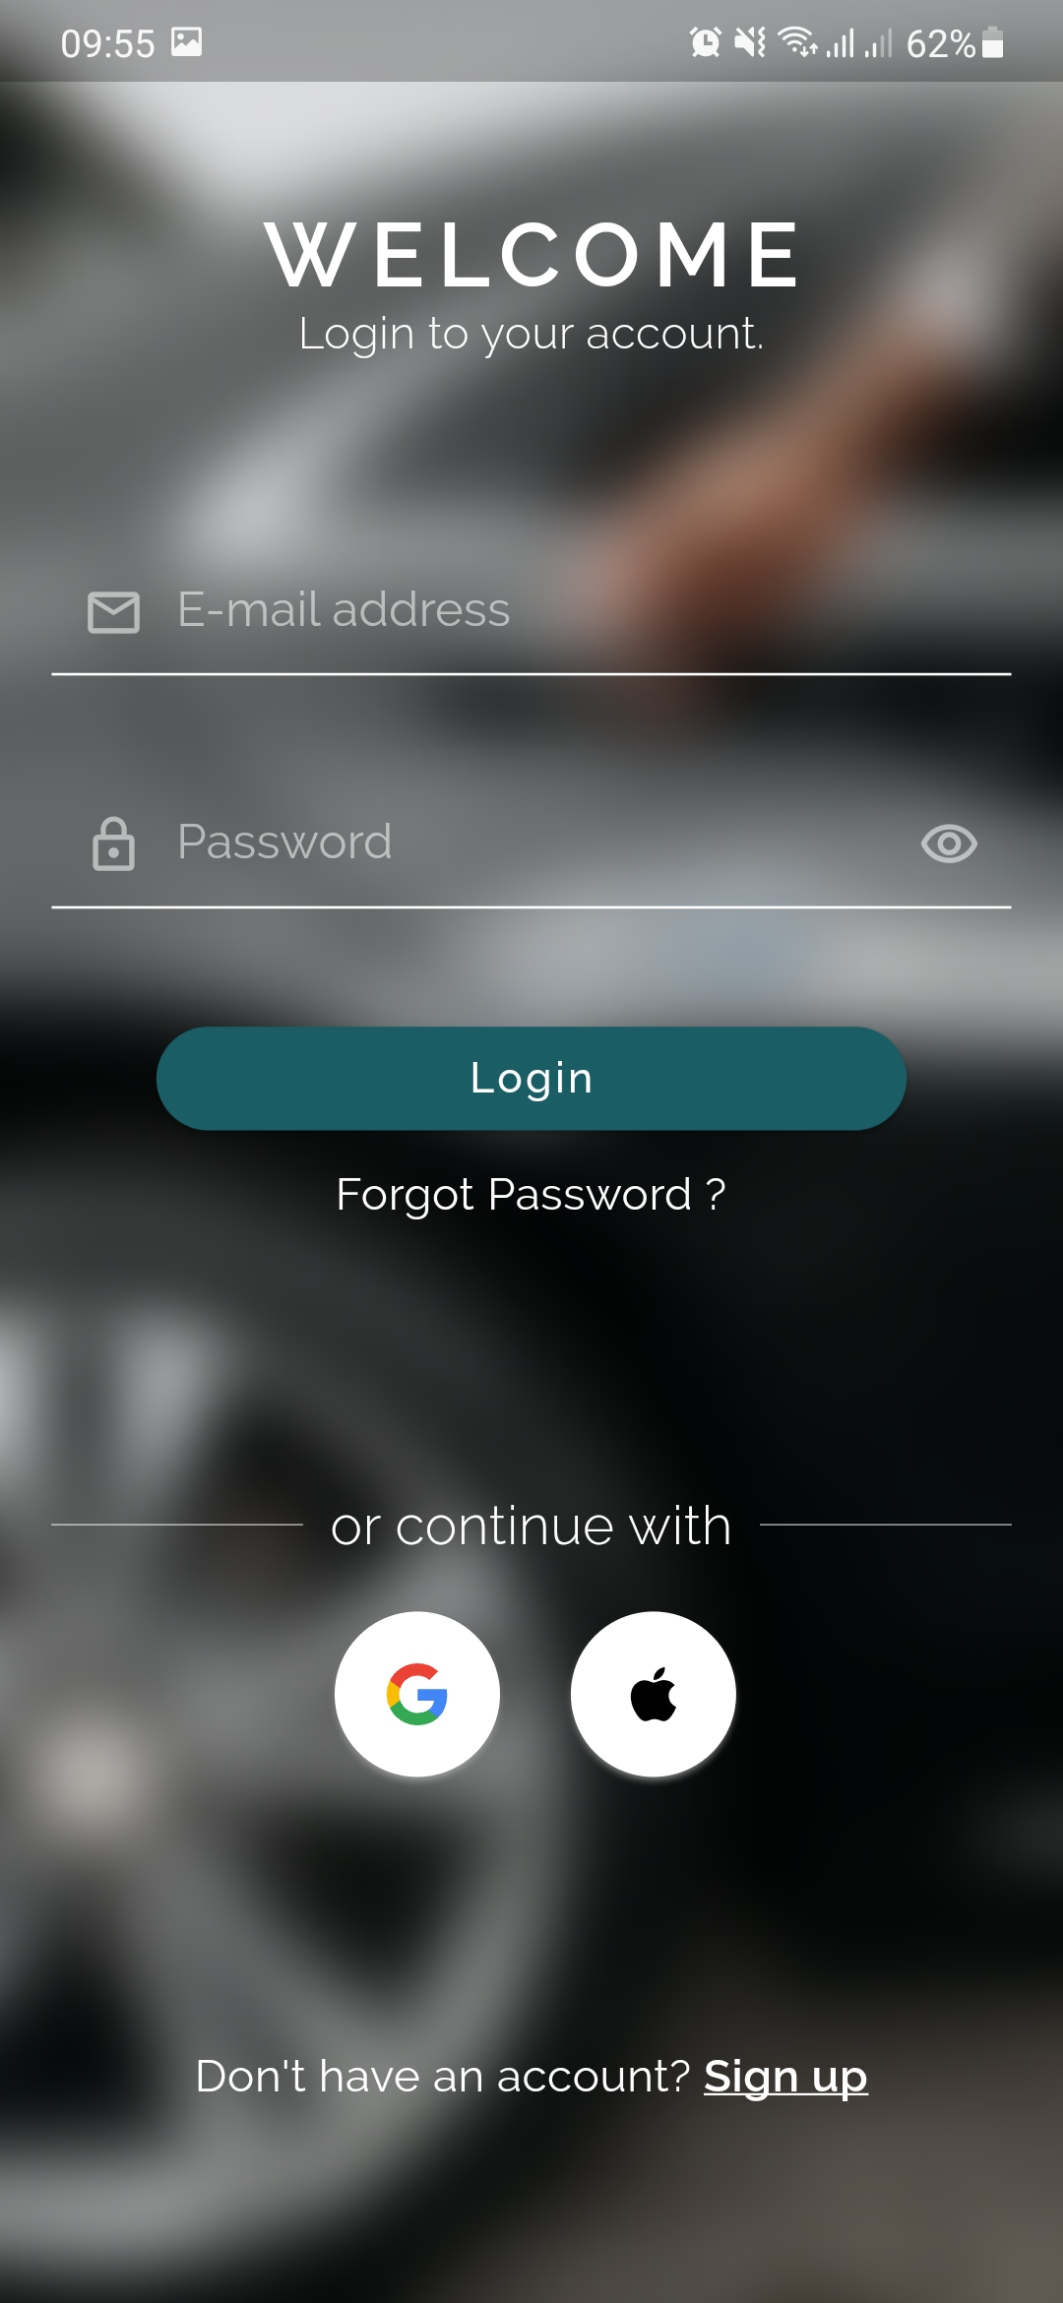
\includegraphics[height = 0.4\textheight]{ui_screenshots/app_screenshots/login_page.png}
            \vspace{1cm}
            \captionsetup{justification=centering}
            \caption{Page de Login.}
            \label{fig:app_login}
        \end{figure}
        \begin{figure}[H]
            \centering
            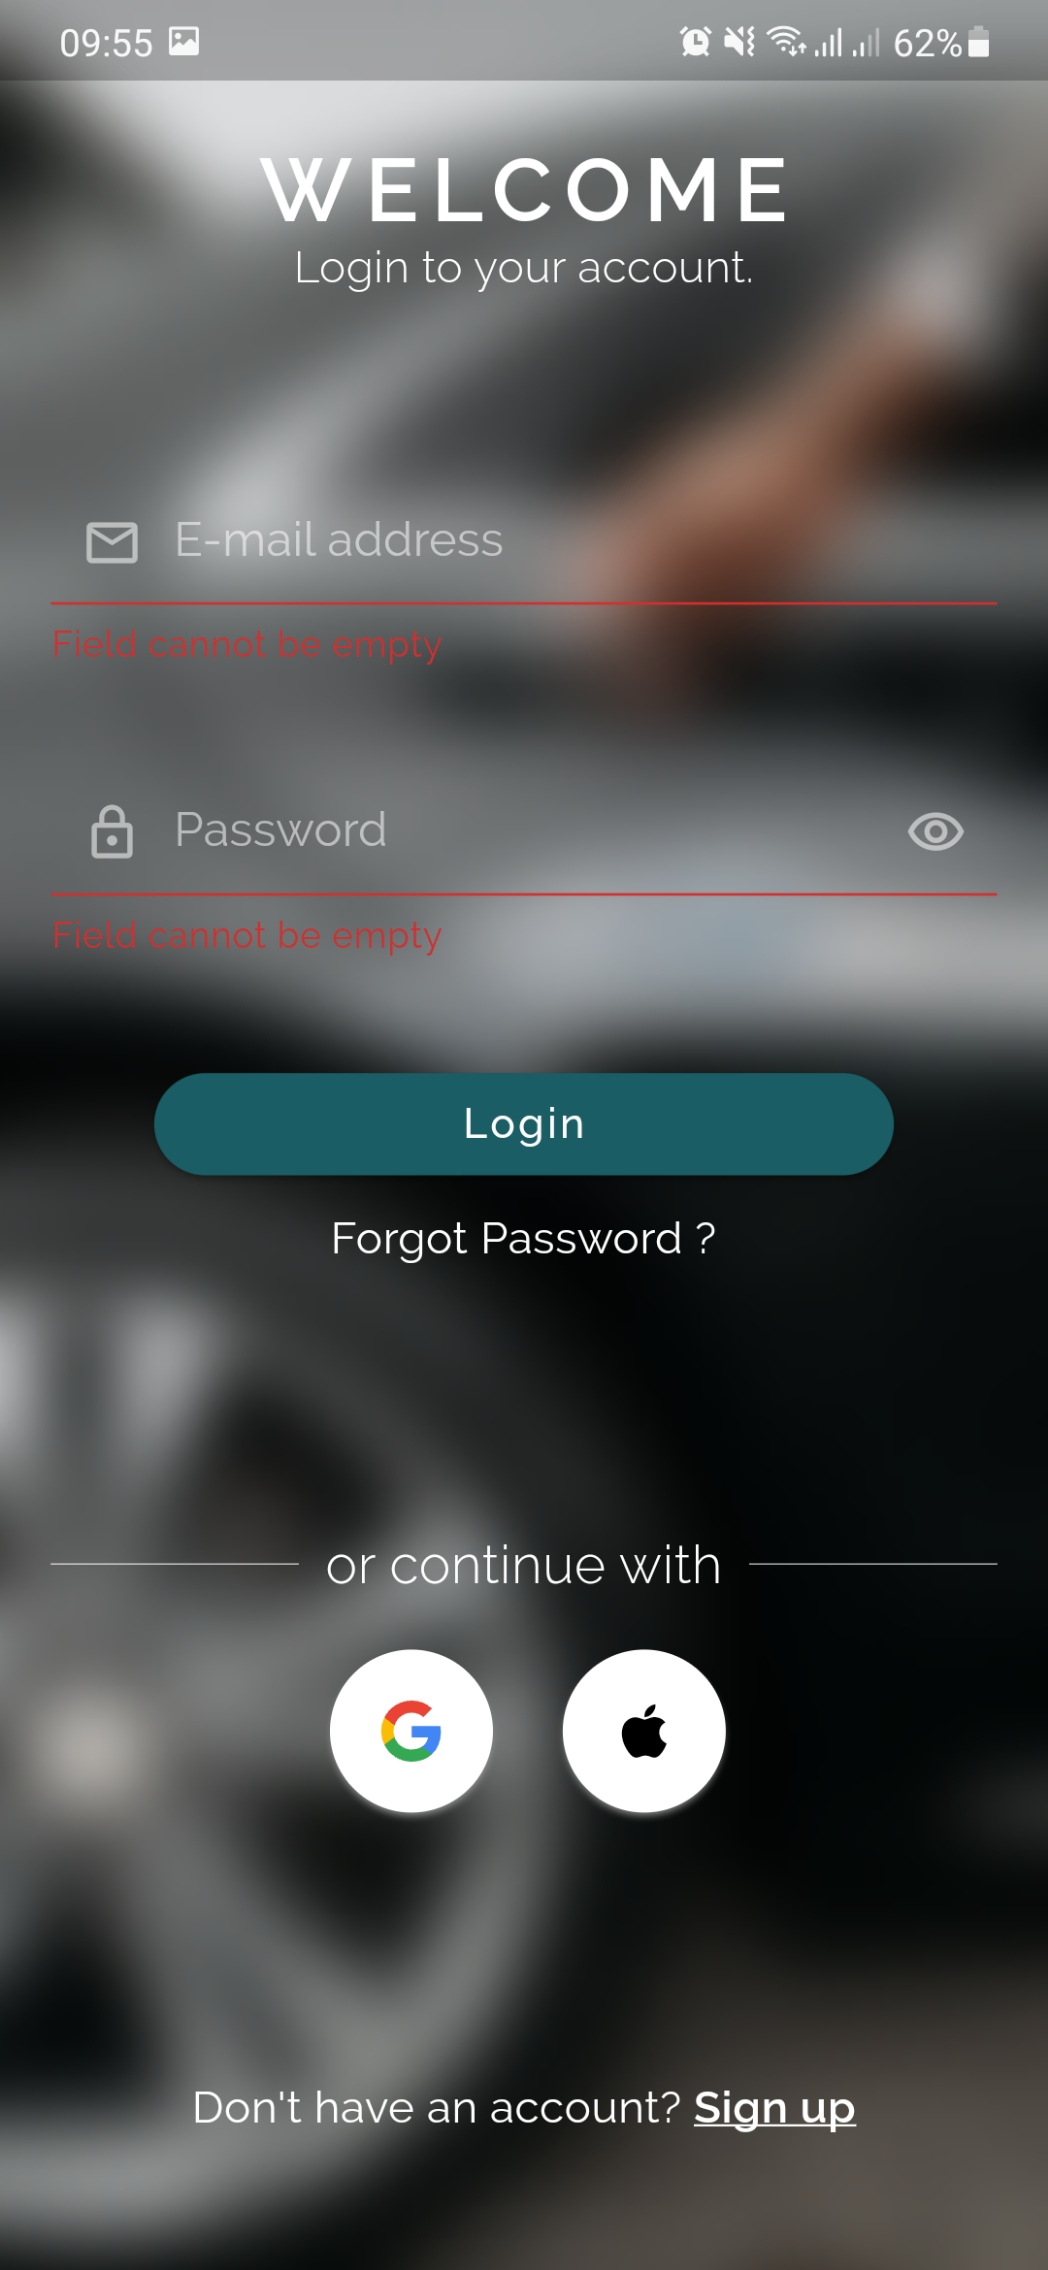
\includegraphics[height = 0.4\textheight]{ui_screenshots/app_screenshots/login_page_validation.png}
            \vspace{1cm}
            \captionsetup{justification=centering}
            \caption{Validation des champs de Login.}
            \label{fig:app_login_validation}
        \end{figure}
    \end{multicols}
\end{center}

\begin{center}
    \begin{figure}[H]
        \centering
        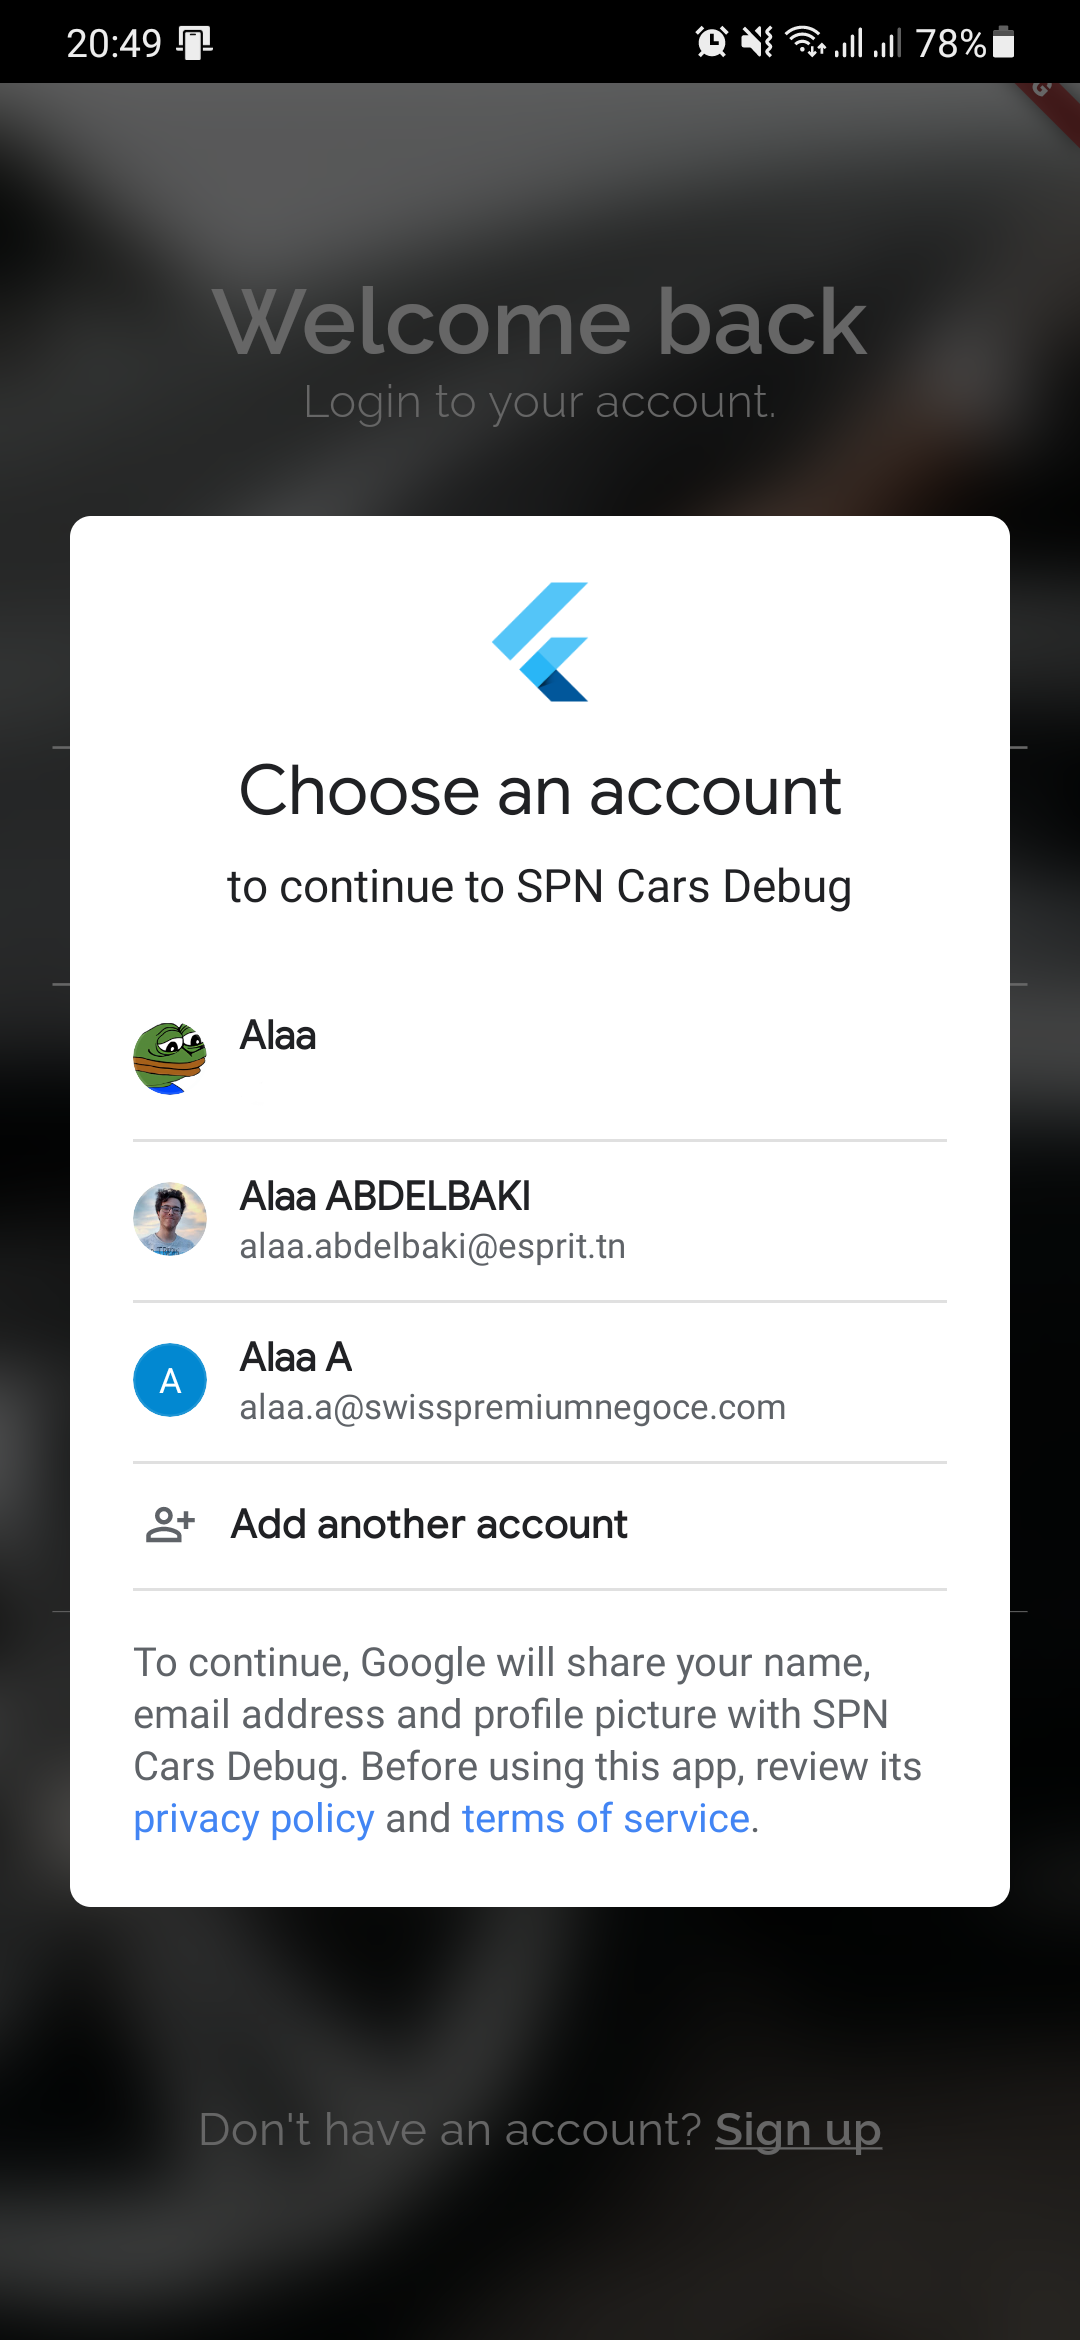
\includegraphics[height = 0.4\textheight]{ui_screenshots/app_screenshots/login_page_google.png}
        \vspace{1cm}
        \captionsetup{justification=centering}

        \caption{Login avec Google.}
        \label{fig:app_login_google}
    \end{figure}
\end{center}
\vspace{1cm}

\section{Page d'accueil}
Une fois l'utilisateur est a réussi à s'authentifier, la page d'accueil s'affiche. Cette page diffère d'un utilisateur à un autre selon les services demandés par l'utilisateur: Si l'utilisateur a un service actif le moment de sa connexion, la liste de voitures louées avec les détails de chaque service actif demandé, et s'il n'a pas de services actif le moment de sa connexion, deux boutons seront affichés : <<Rent a car>> pour louer une voiture sans chauffeur et <<Request a transfer>> pour demander un chauffeur avec une voiture.
\vspace{1cm}
\clearpage
\begin{multicols}{2}
    \begin{figure}[H]
        \centering
        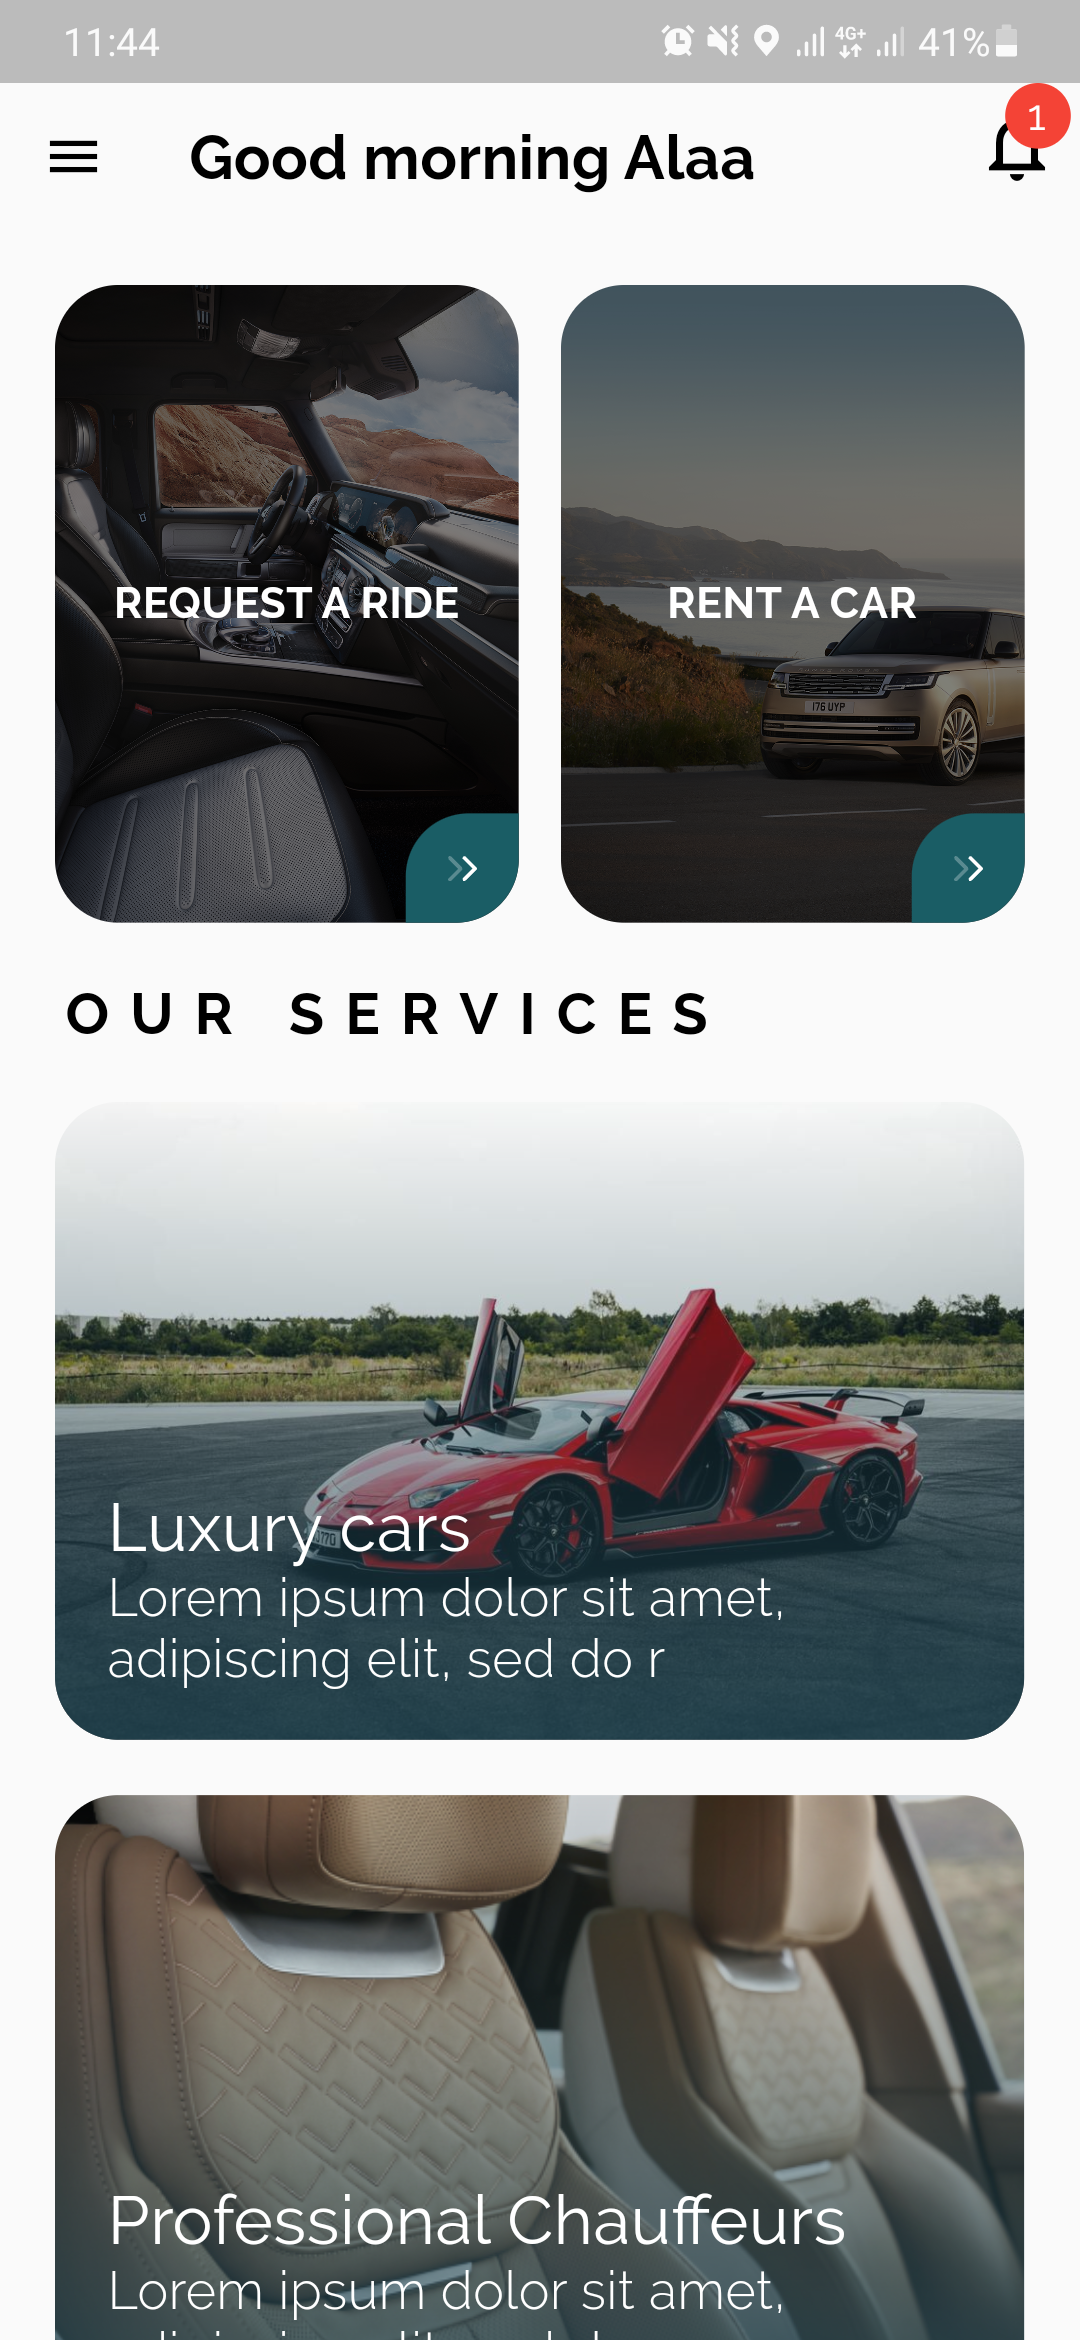
\includegraphics[height = 0.4\textheight]{ui_screenshots/app_screenshots/Home_1.png}
        \vspace{1cm}
        \captionsetup{justification=centering}
        \caption{Page d'accueil sans réservation active.}
        \label{fig:home_no_res}
    \end{figure}
    \begin{figure}[H]
        \centering
        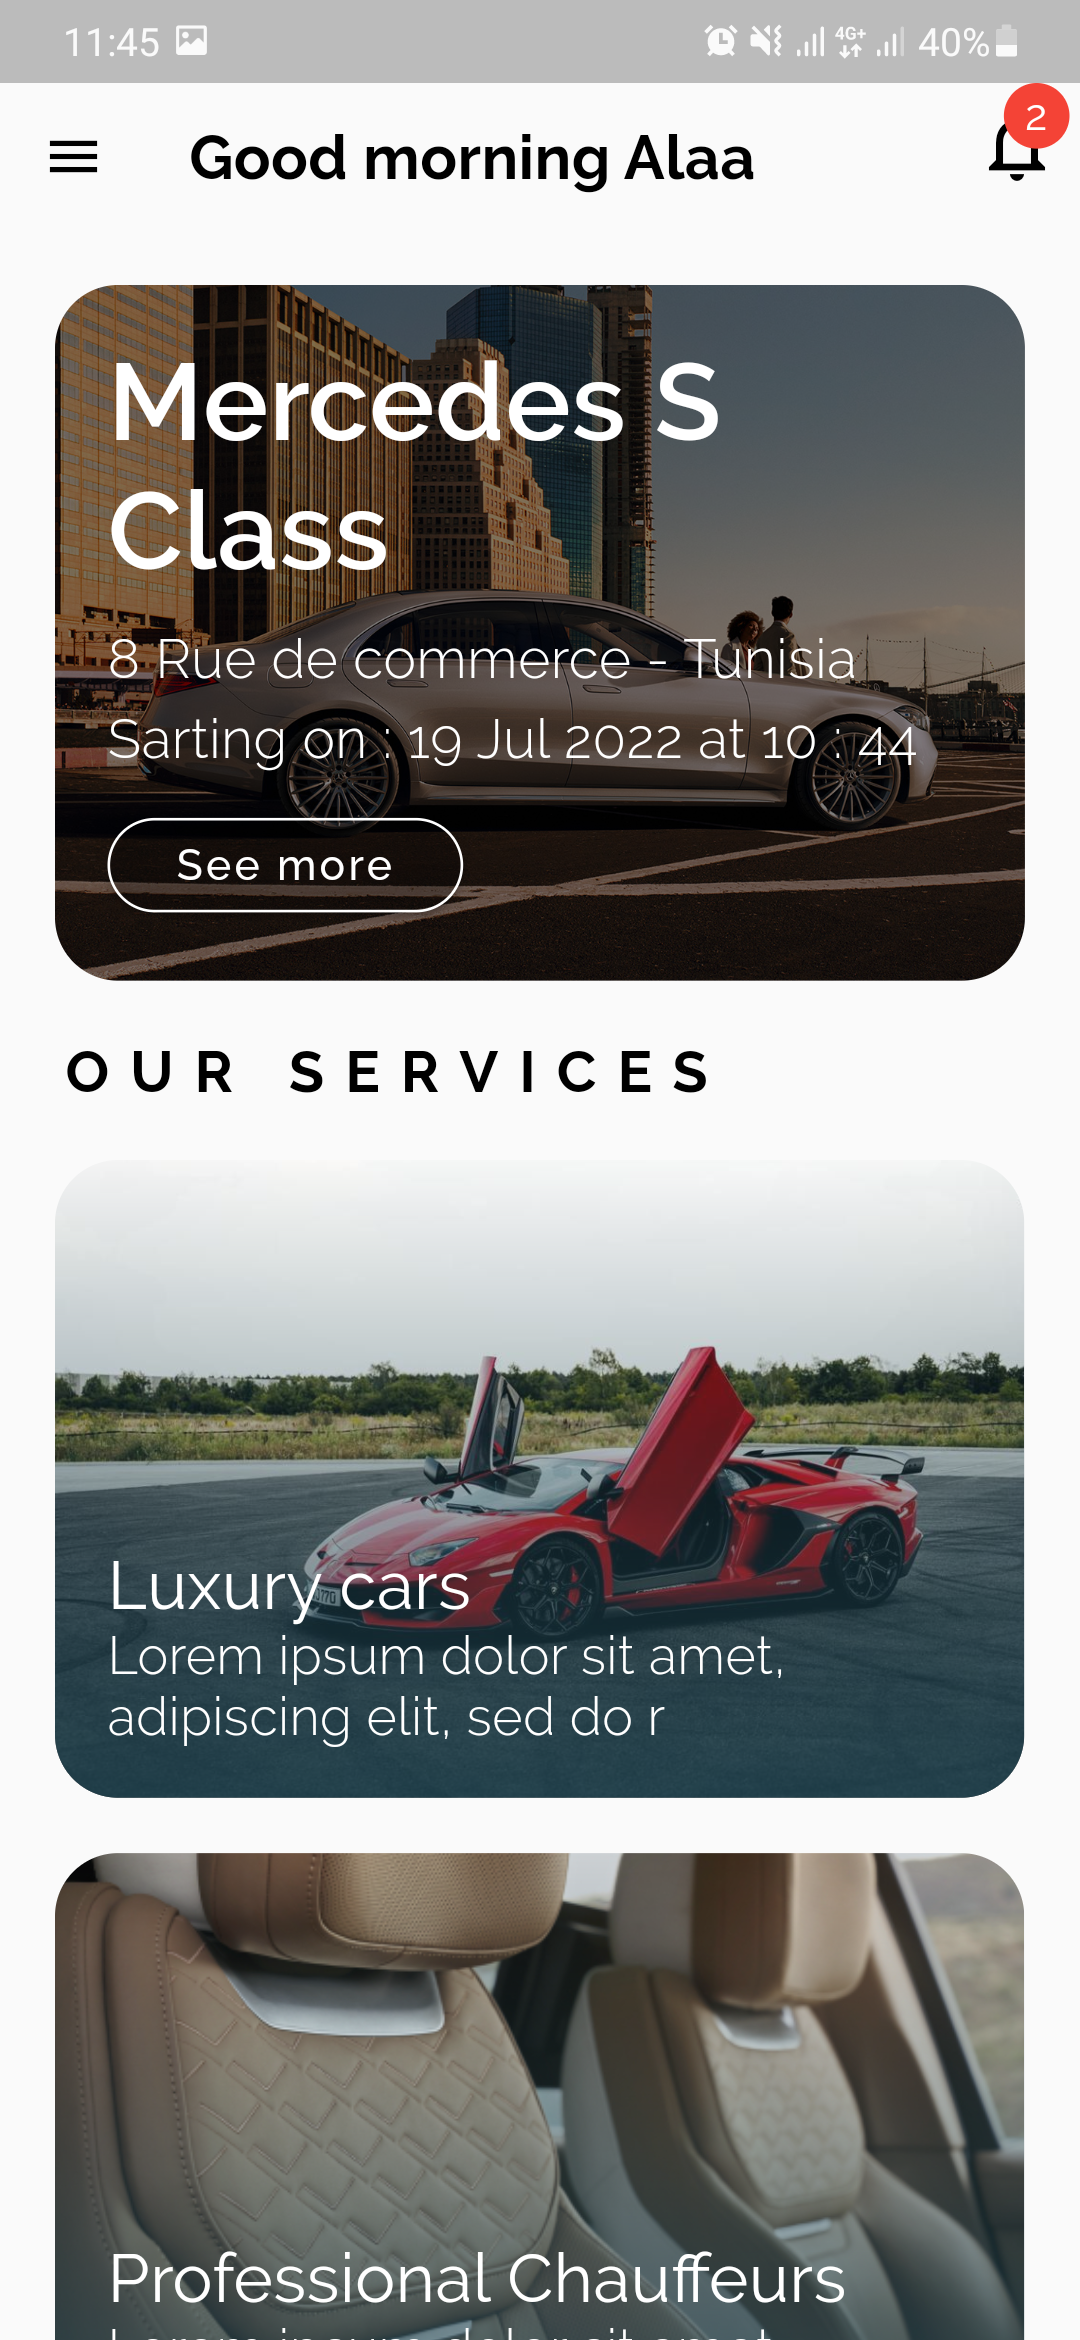
\includegraphics[height = 0.4\textheight]{ui_screenshots/app_screenshots/Home_2.png}
        \vspace{1cm}
        \captionsetup{justification=centering}
        \caption{Page d'accueil avec réservation active.}
        \label{fig:home_res}
    \end{figure}
\end{multicols}
\vspace{1cm}
\section{Gestion de profil}
Chaque utilisateur possède un profil personnel, ce profil affichera les informations nécessaires pour faciliter la communication entre utilisateurs dans le futur (Ex: Contact entre chauffuer et client).\\
\noindent La page de profil, dans l'application SPN-Cars, est une page très simple qui contient les informations de base de l'utilisateur :
\begin{itemize}
    \item La photo de profil.
    \item Le nom.
    \item Le prénom
    \item L'adresse E-mail.
    \item Le numéro de téléphone.
    \item La date de naissance.
\end{itemize}
De toutes ses données seuls le nom, prénom, photo de profil et numéro de téléphone seront accessibles aux chauffeurs pour assurer une communication avec les clients.\\
\noindent L'utilisateur peut modifier tous ses informations personnelles tout simplement en modifiant les champs contenant l'information à changer, et pour la photo de profile il suffit d'appuyer sur la photo pour la remplacer par une autre, soit prendre une nouvelle photo en utilisant l'appareil photo du smartphone, ou en choisissant une photo existante depuis la galerie. Une fois l'image est choisie, l'utilisateur sera redirigé vers une page pour recadrer l'image et choisir la zone qui sera affichée dans la page de profile, une fois l'image est recadrée, elle sera compressée pour réduire sa taille et faciliter son transfert vers le serveur distant.
\begin{figure}[H]
    \centering
    \includegraphics[height = 0.4\textheight]{ui_screenshots/app_screenshots/profile.png}
    \vspace{1cm}
    \captionsetup{justification=centering}
    \caption{Page de gestion de profil.}
    \label{fig:prifle}
\end{figure}
\section{Demander un service}
Pour louer une voiture, l'utilisateur a besoin de spécifier tout d'abord les paramètres suivants :
\begin{itemize}
    \item Le type de service demandé (Location / Transfert / Excursion / Long Ride).
    \item L'adresse de départ.
    \item L'heure de départ.
    \item L'adresse d'arrivée (Pas toujours disponible selon le type de service).
    \item L'heure d'arrivée (Pas toujours disponible selon le type de service).
    \item La durée du service demandé (Pas toujours disponible selon le type de service).
\end{itemize}
\vspace{1cm}
\clearpage
\vspace{1cm}
\begin{multicols}{2}
    \begin{figure}[H]
        \centering
        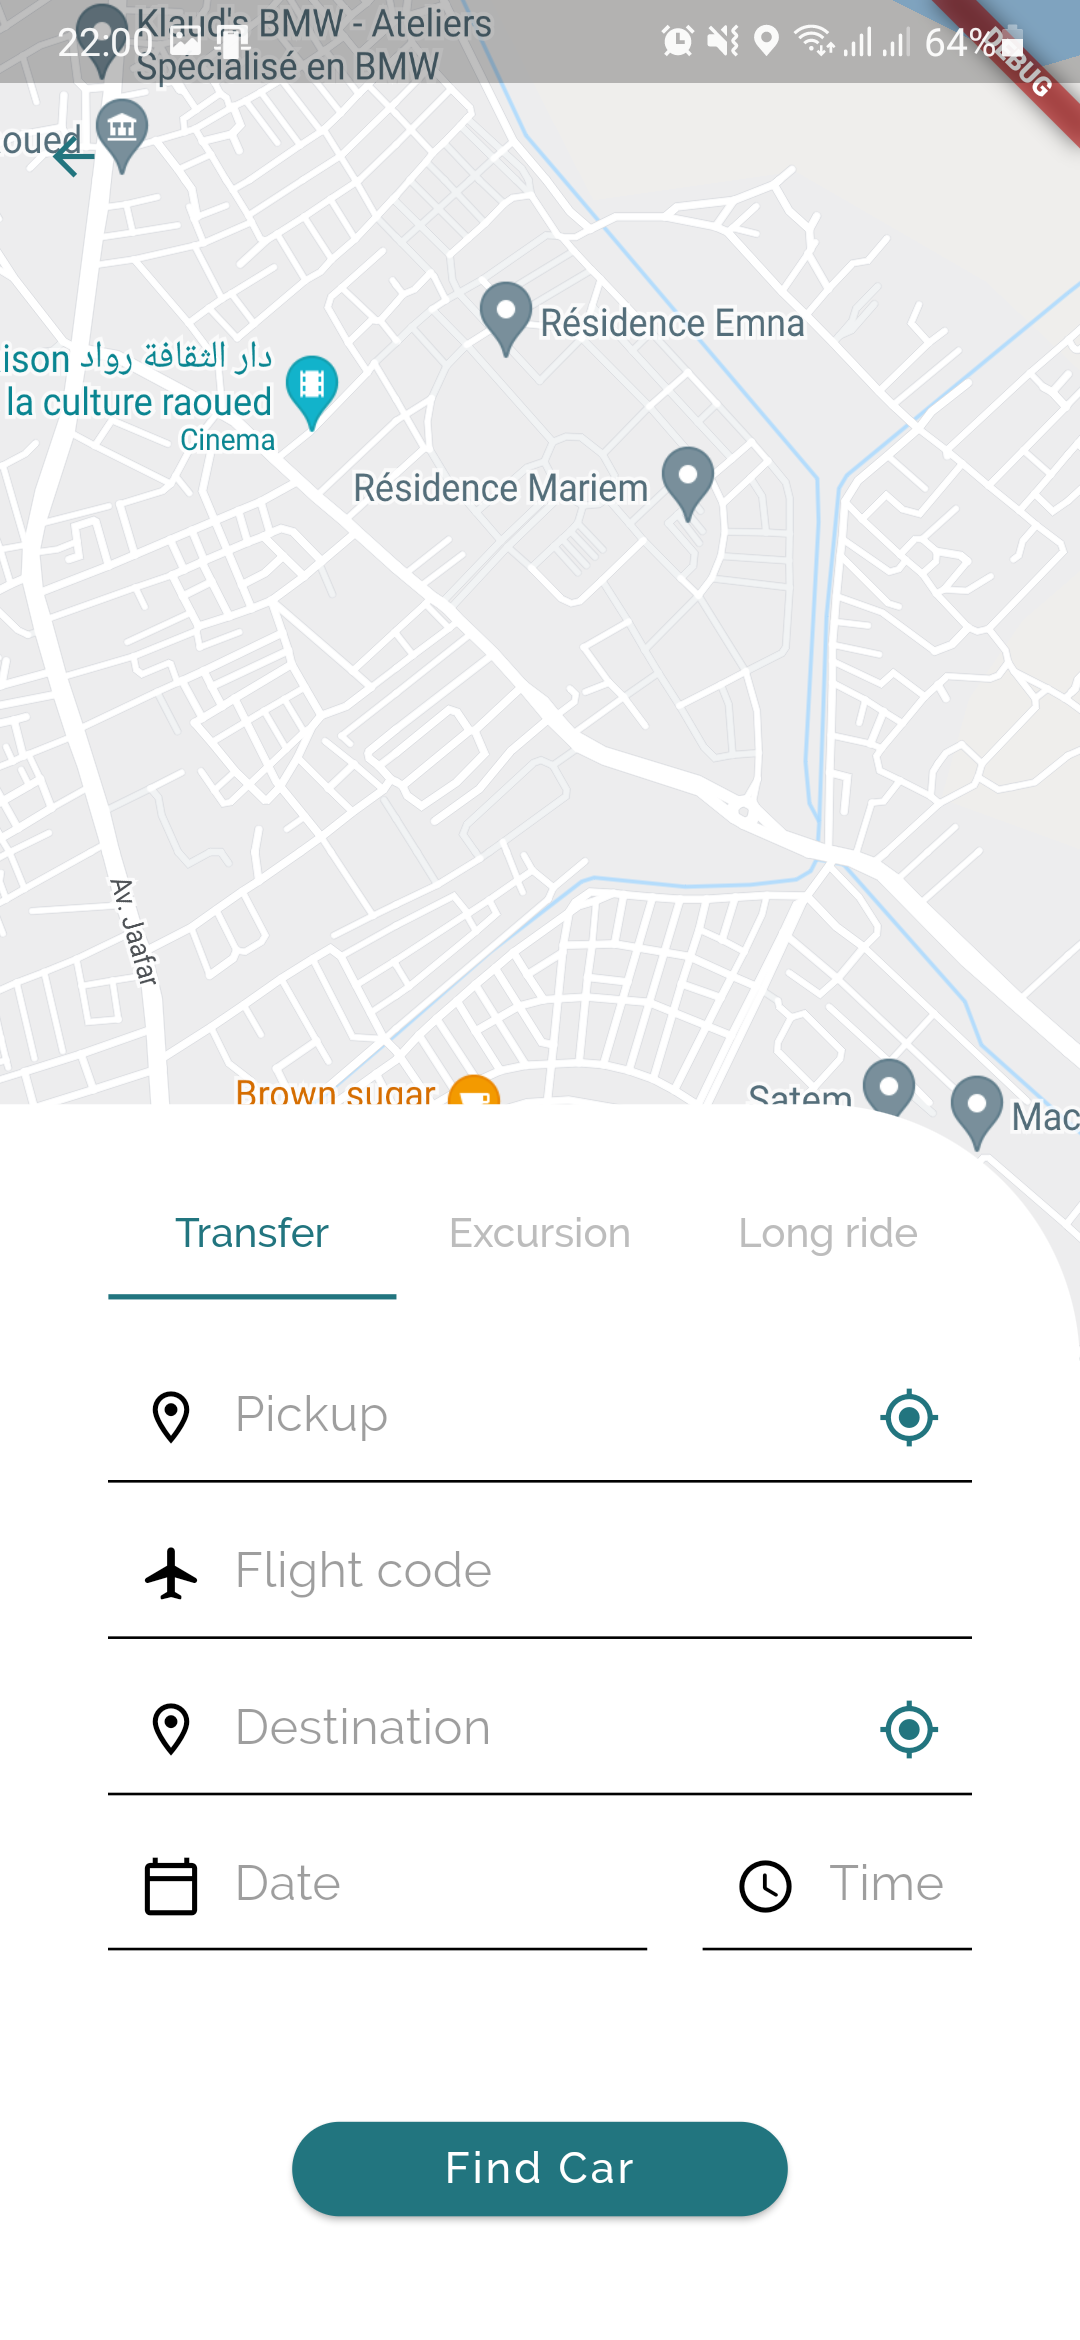
\includegraphics[height = 0.4\textheight]{ui_screenshots/app_screenshots/transfer_form.png}
        \captionsetup{justification=centering}
        \caption{Formulaire de demande de transfert.}
        \label{fig:app_transfer}
    \end{figure}
    \begin{figure}[H]
        \centering
        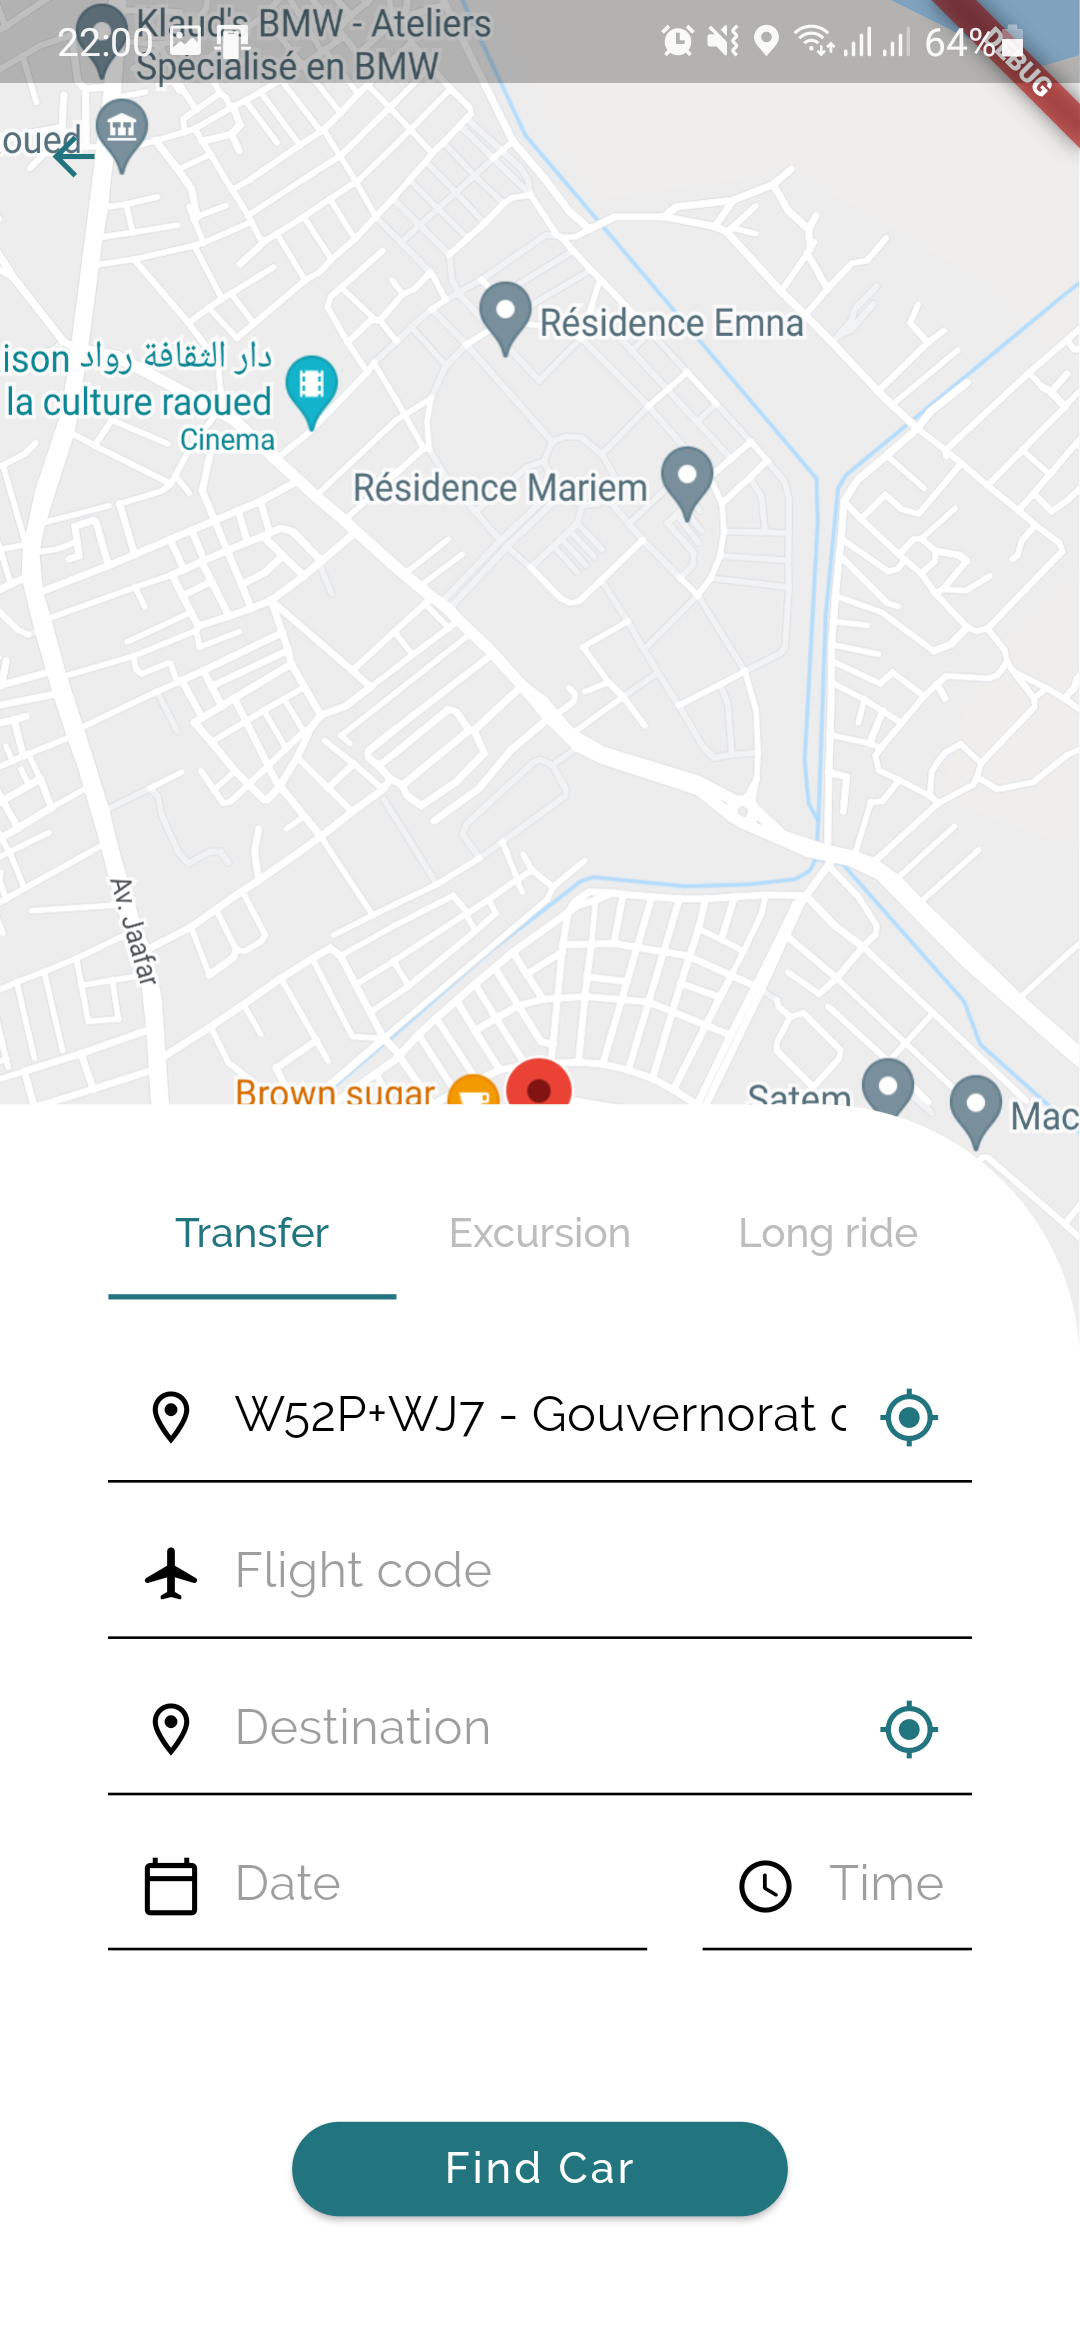
\includegraphics[height = 0.4\textheight]{ui_screenshots/app_screenshots/current_location.png}
        \captionsetup{justification=centering}
        \caption{Utiliser le bouton <<Localiser>> pour choisir la position actuelle.}
        \label{fig:app_transfer_current_pos}
    \end{figure}
\end{multicols}
\begin{multicols}{2}
    \begin{figure}[H]
        \centering
        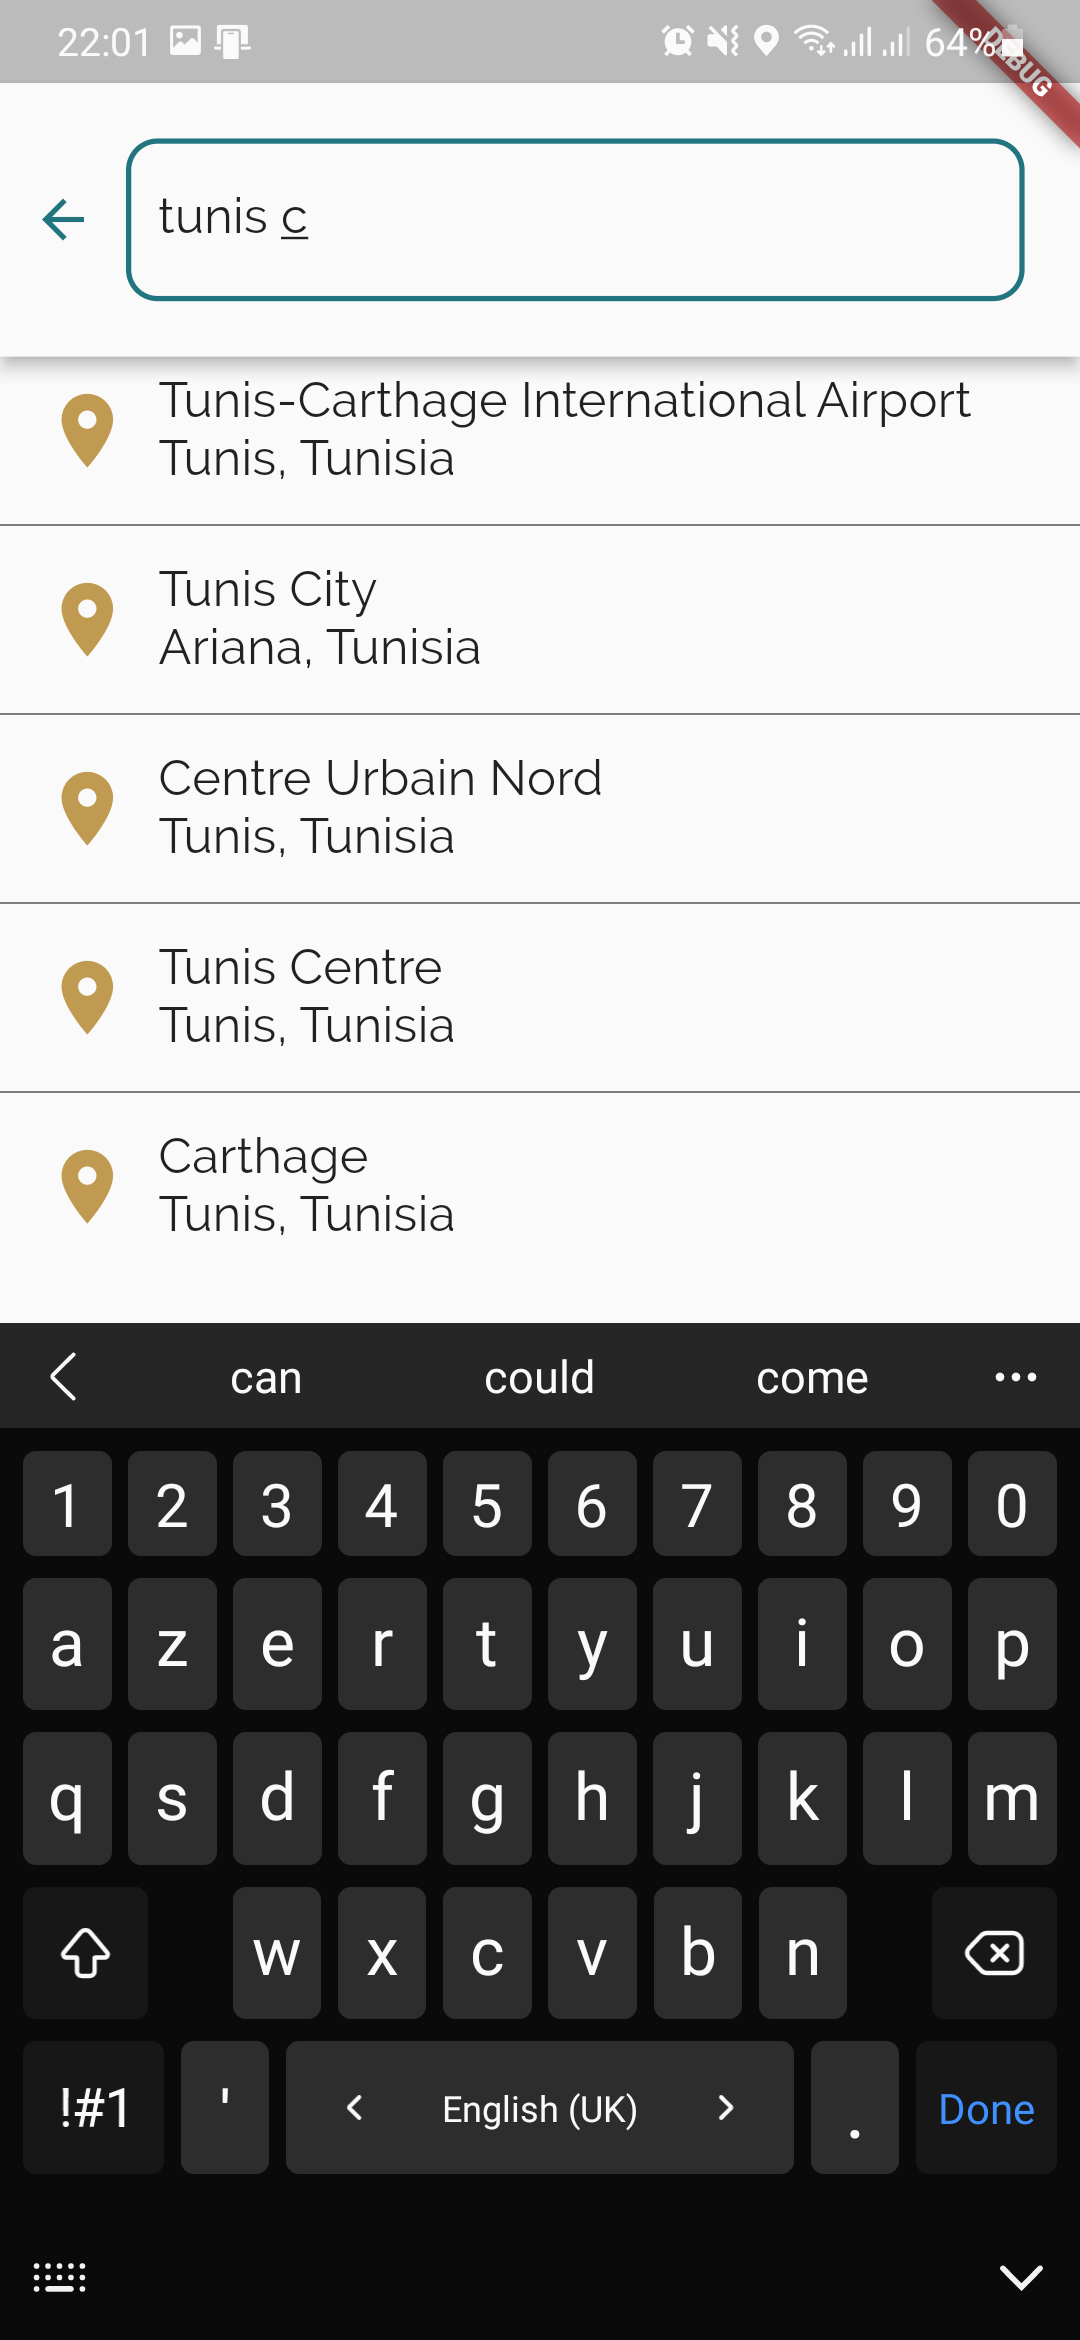
\includegraphics[height = 0.4\textheight]{ui_screenshots/app_screenshots/suggestions.png}
        \captionsetup{justification=centering}
        \caption{Rechercher un emplacement à l'aide de Google Places.}
        \label{fig:app_transfer_suggestions}
    \end{figure}
    \begin{figure}[H]
        \centering
        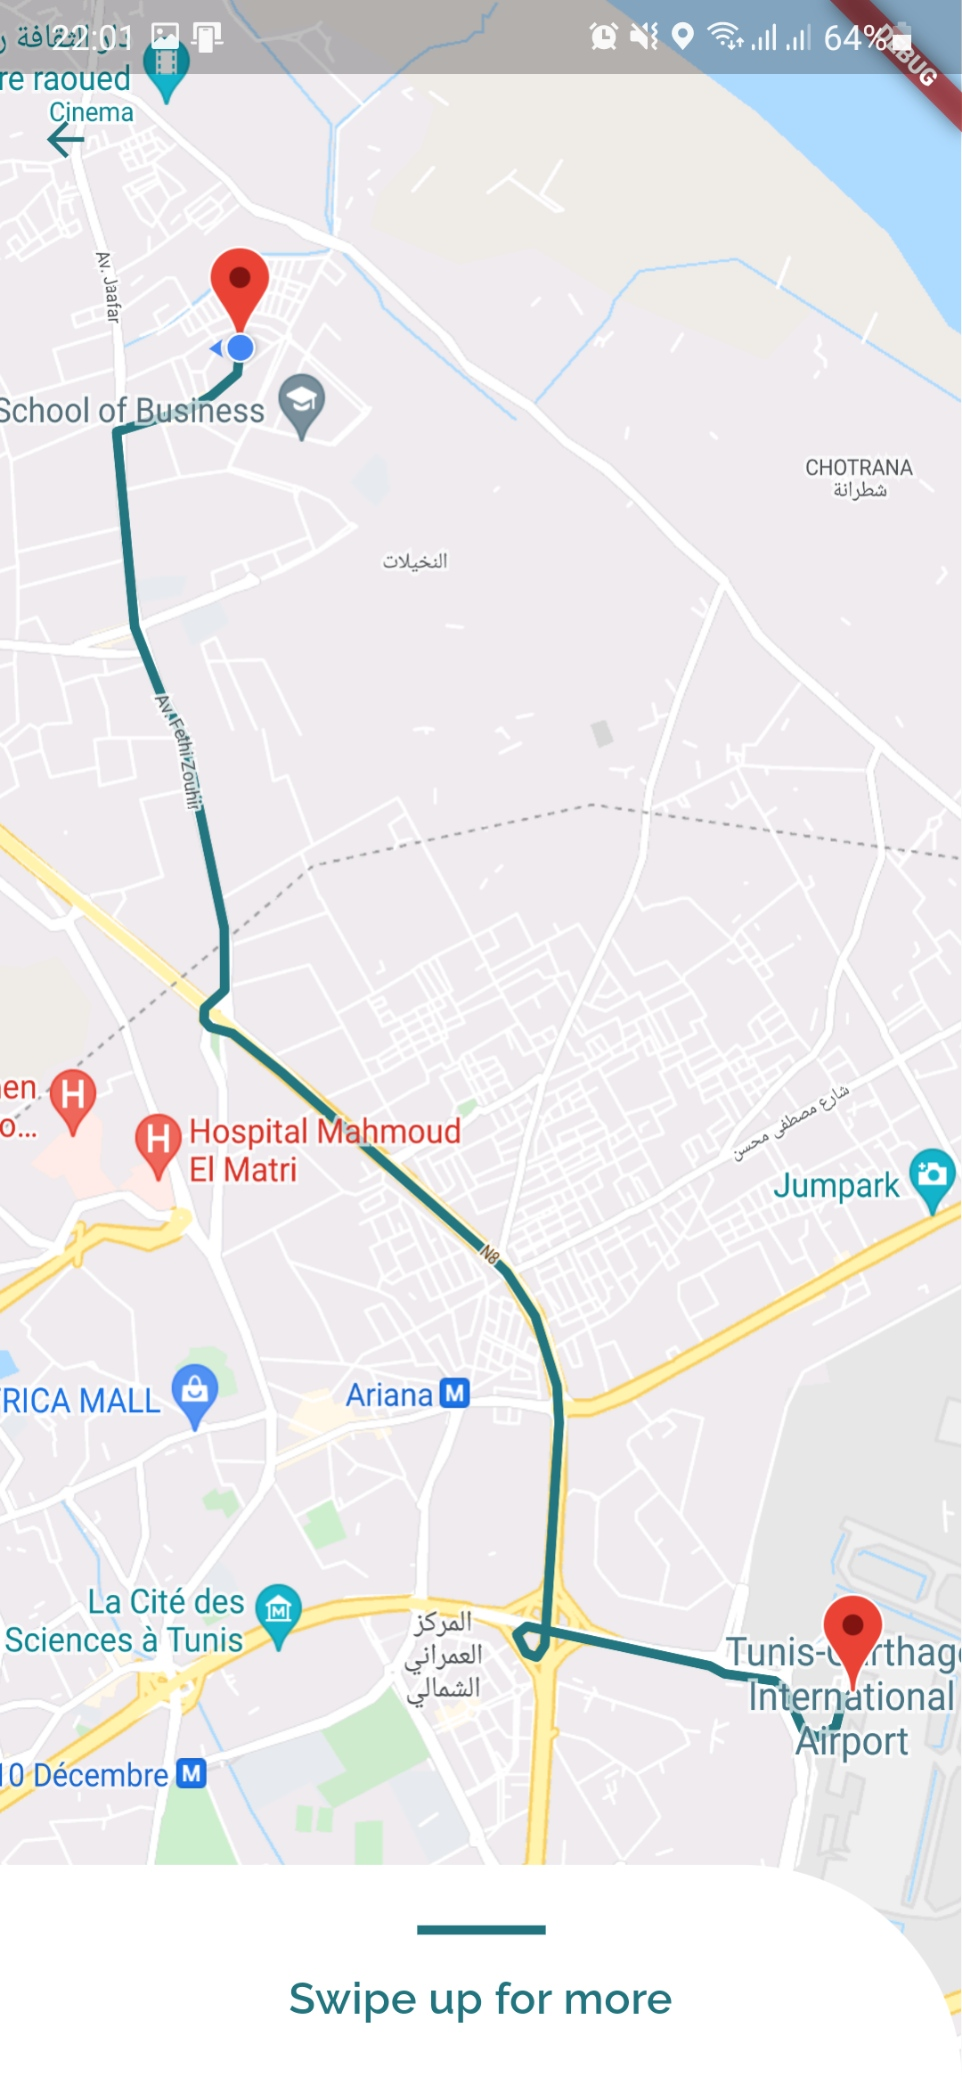
\includegraphics[height = 0.4\textheight]{ui_screenshots/app_screenshots/directions.png}
        \captionsetup{justification=centering}
        \caption{Afficher la meilleure route entre le point de départ et le point d'arrivée.}
        \label{fig:app_transfer_directions}
    \end{figure}
\end{multicols}
\section{Affichage des voitures disponibles}
Après sélection des informations nécessaires par l'utilisateur, une recherche des voitures qui répondent aux critères de recherche choisis. Une fois qu'une liste de voitures est prête, les voitures seront affichées. L'utilisateur peut appuyer sur une voiture pour découvrir ses caractéristiques et choisir ensuite de la louer ou continuer sa recherche.
\begin{multicols}{2}
    \begin{figure}[H]
        \centering
        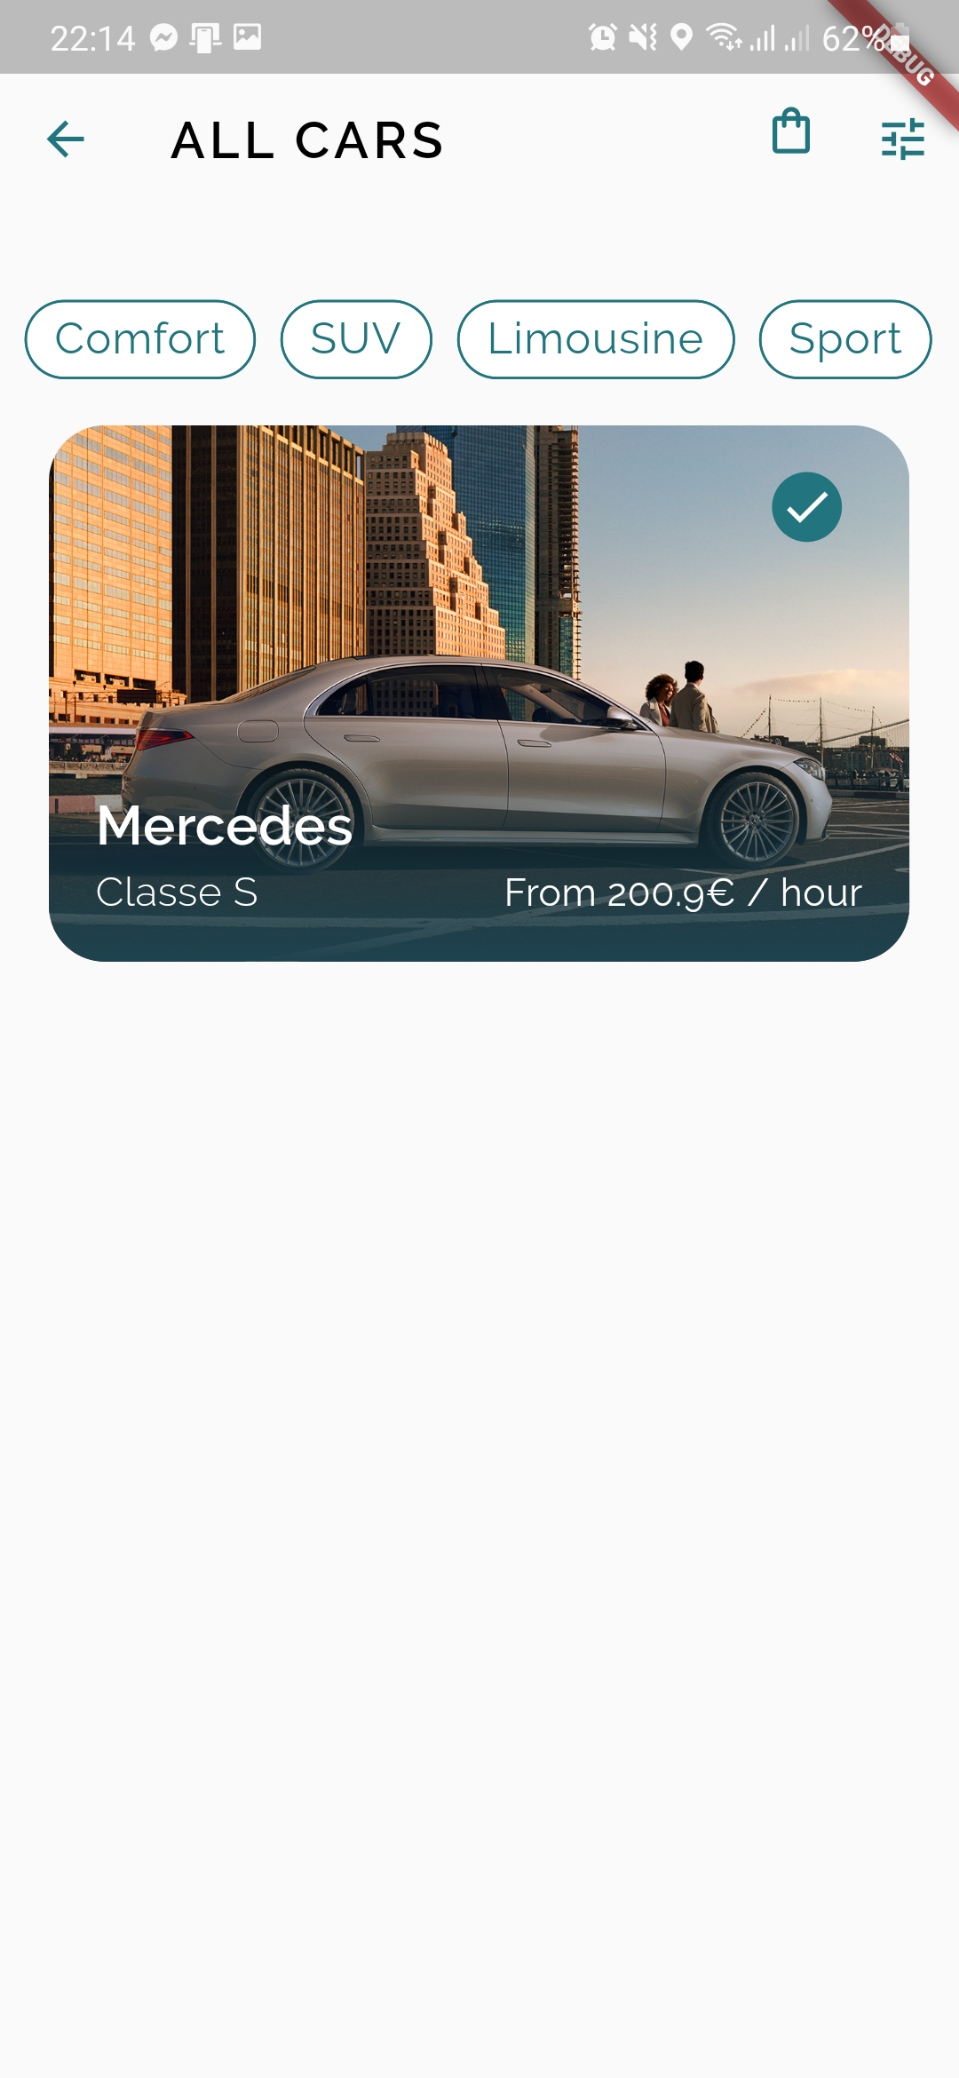
\includegraphics[height = 0.4\textheight]{ui_screenshots/app_screenshots/available_cars.png}
        \captionsetup{justification=centering}
        \caption{Liste des voitures disponibles selon le point de départ sélectionné.}
        \label{fig:app_available_cars}
    \end{figure}
    \begin{figure}[H]
        \centering
        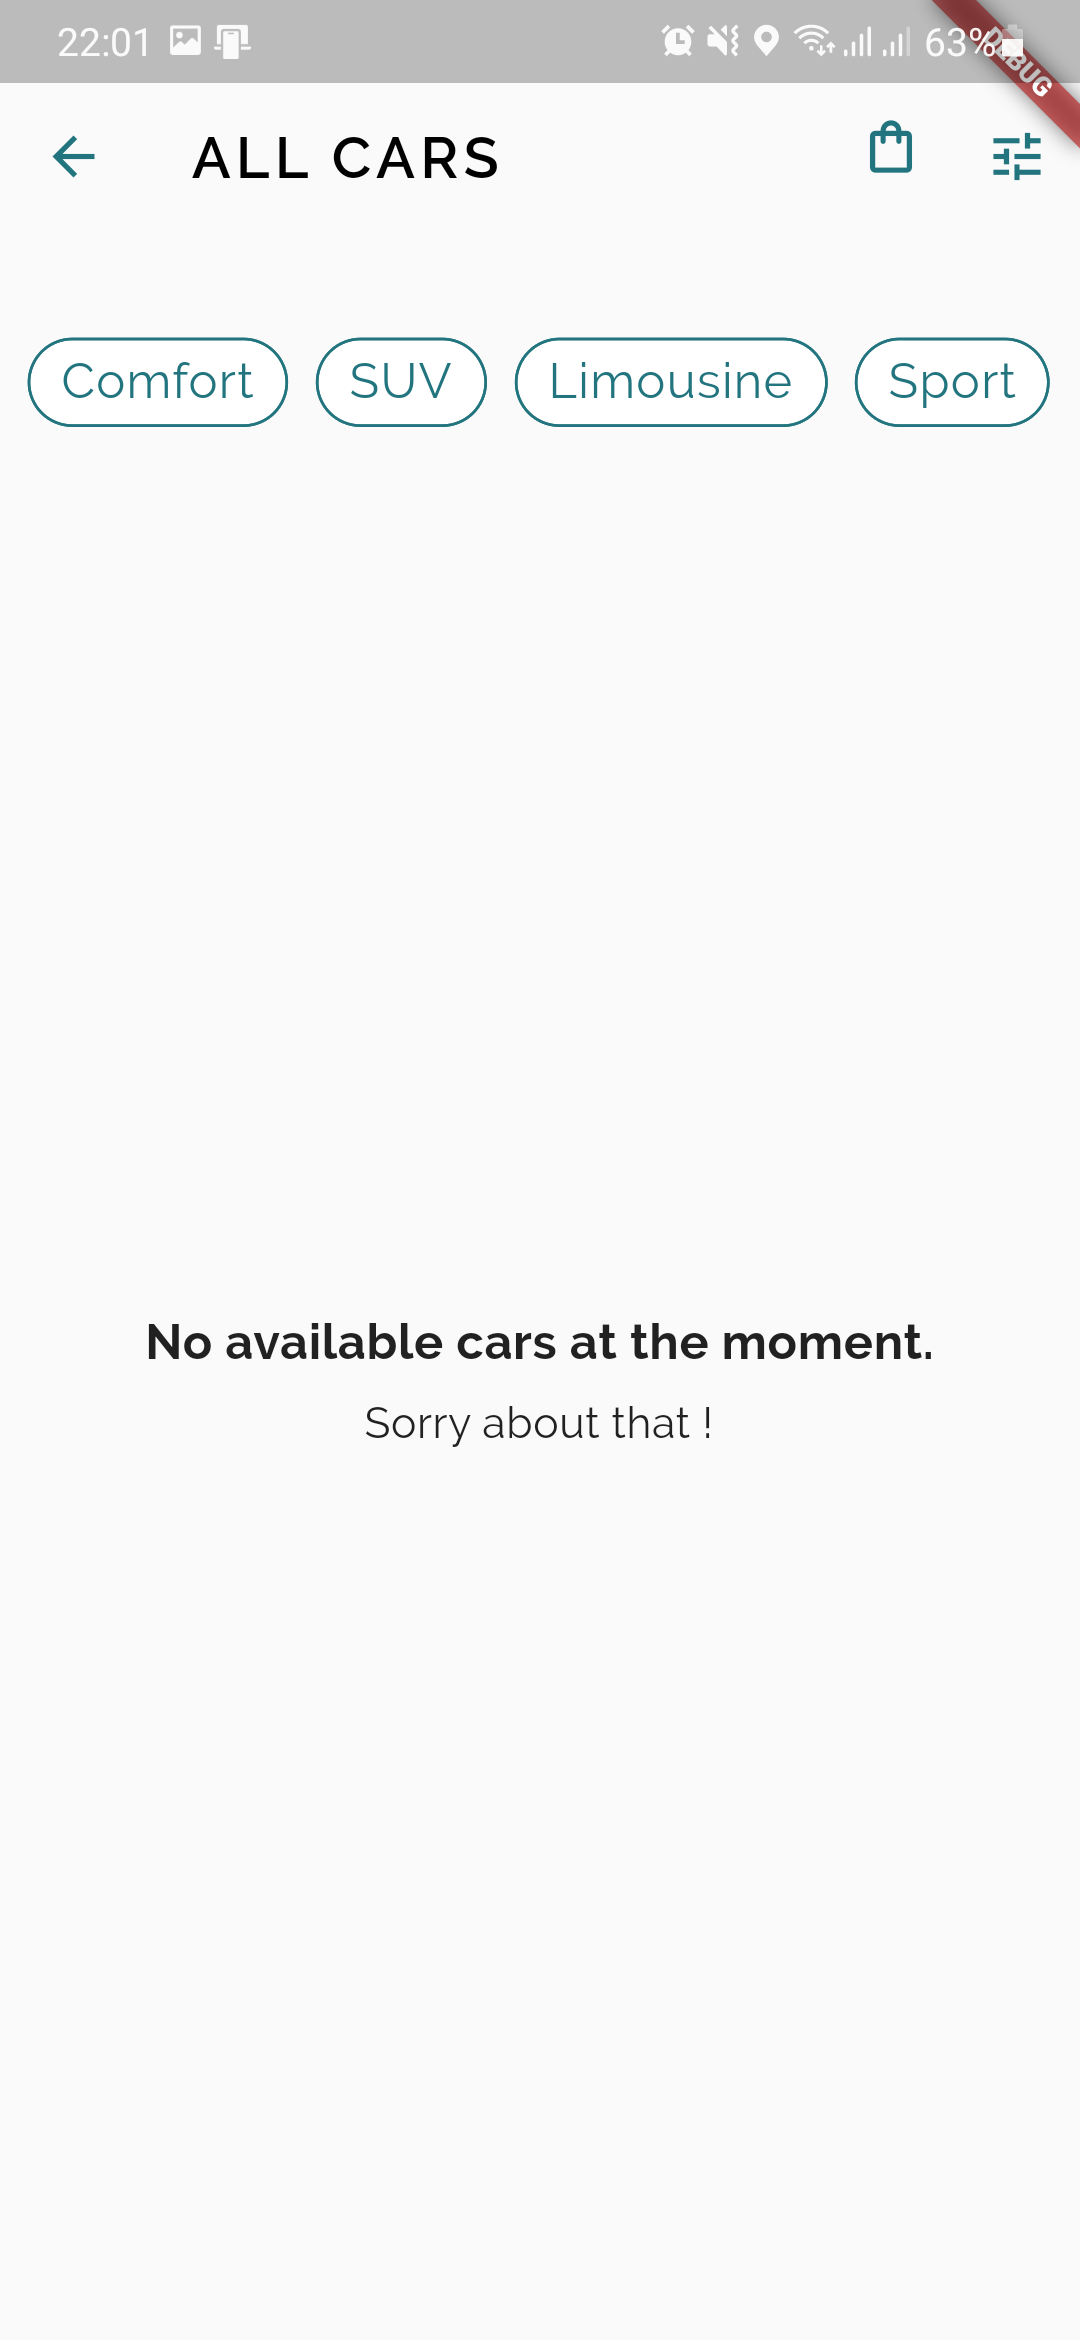
\includegraphics[height = 0.4\textheight]{ui_screenshots/app_screenshots/available_cars_empty.png}
        \captionsetup{justification=centering}
        \caption{Affichage si aucune voiture n'est disponible.}
        \label{fig:app_available_cars_empty}
    \end{figure}
\end{multicols}
\section{Signature numérique de contrat de location}
Pour le cas de location de voitures, un contrat doit être signé entre le client et la société. Pour s'assurer de la signature du contrat, on a opté pour la solution de signature numérique à l'aide du service offert par DocuSign, qui se spécialise dans le domaine de la signature électronique et la gestion des transactions numériques pour faciliter les échanges et les validations électroniques des contrats et de documents.\\
\noindent Pour créer une réservation de location de voitures, il suffit d'appuyer sur le bouton de <<Book now>> dans la page de détails de la voiture choisie, et une réservation sera créée avec tous les détails : La position GPS, la date de récupération et retour de voiture et les informations de contact du client. Une fois ses informations sont enregistrées, un email contenant le contrat sera envoyé au client pour le signer, et l'identifiant de ce contrat sera enregistré avec les informations de la réservation.\\
\noindent Dans l'application, le client est redirigé vers la page de vérification de signature où il doit appuyer sur le bouton de vérification de l'état de contrat. Pour signer ce contrat, il suffit d'ouvrir le document envoyé à l'adresse email du client, le signer, et retourner vers l'application. Lors de l'appui sur le bouton <<Verify Signature>>, une requête sera envoyée au back-end qui contactera les APIs de <<DocuSign>> pour vérifier l'état de signature du contrat à l'aide de l'identifiant du contrat fourni lors de la création de la réservation. Si l'état de contrat est <<sent>>, le contrat n'est pas encore signé, et un message d'erreur sera affiché à l'utilisateur. Sinon si l'état du contrat est <<completed>>, les contrat est, donc, signé et l'utilisateur est redirigé vers la page de paiement.
\vspace{1cm}

\begin{multicols}{2}
    \begin{figure}[H]
        \centering
        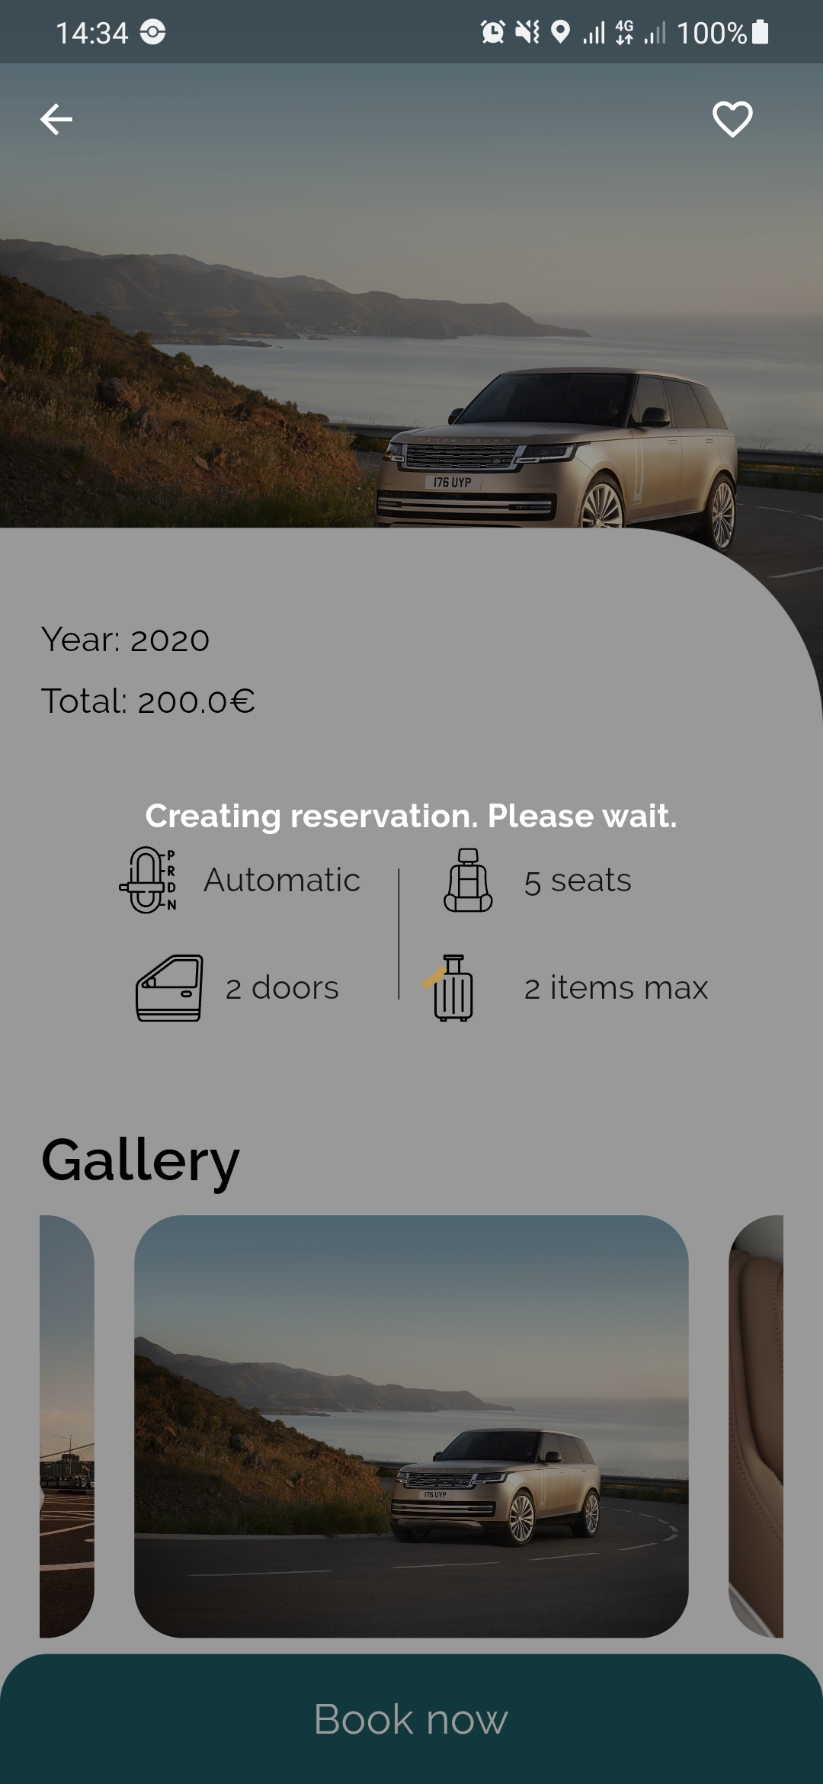
\includegraphics[height = 0.4\textheight]{ui_screenshots/app_screenshots/create_reservation.png}
        \captionsetup{justification=centering}
        \caption{Création de réservation.}
        \label{fig:create_res}
    \end{figure}
    \begin{figure}[H]
        \centering
        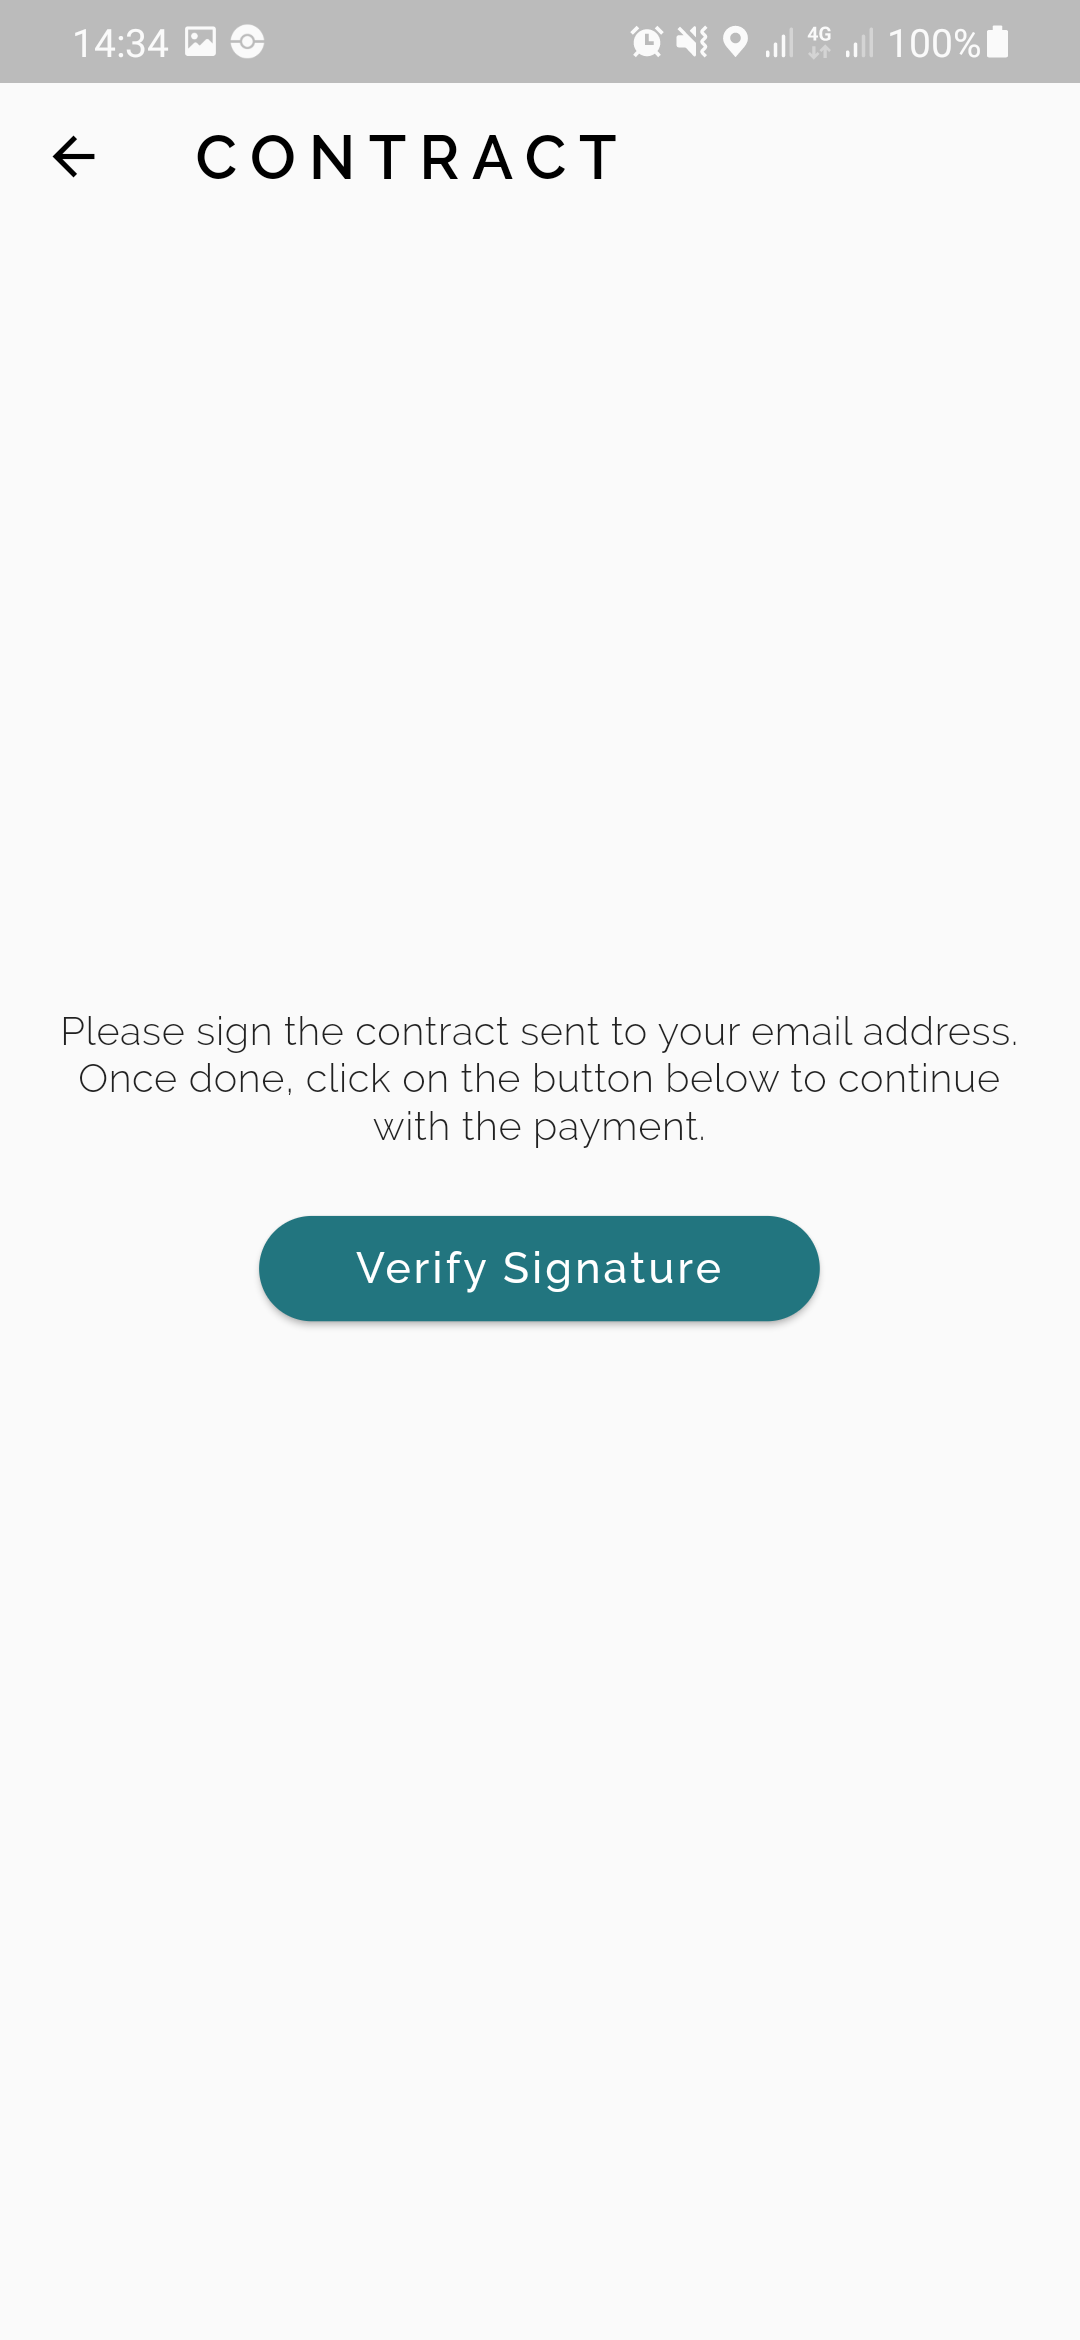
\includegraphics[height = 0.4\textheight]{ui_screenshots/app_screenshots/verify_sig.png}
        \captionsetup{justification=centering}
        \caption{Page de vérification de signature}
        \label{fig:verify_sig}
    \end{figure}
\end{multicols}
\vspace{1cm}
\clearpage
\begin{multicols}{2}
    \begin{figure}[H]
        \centering
        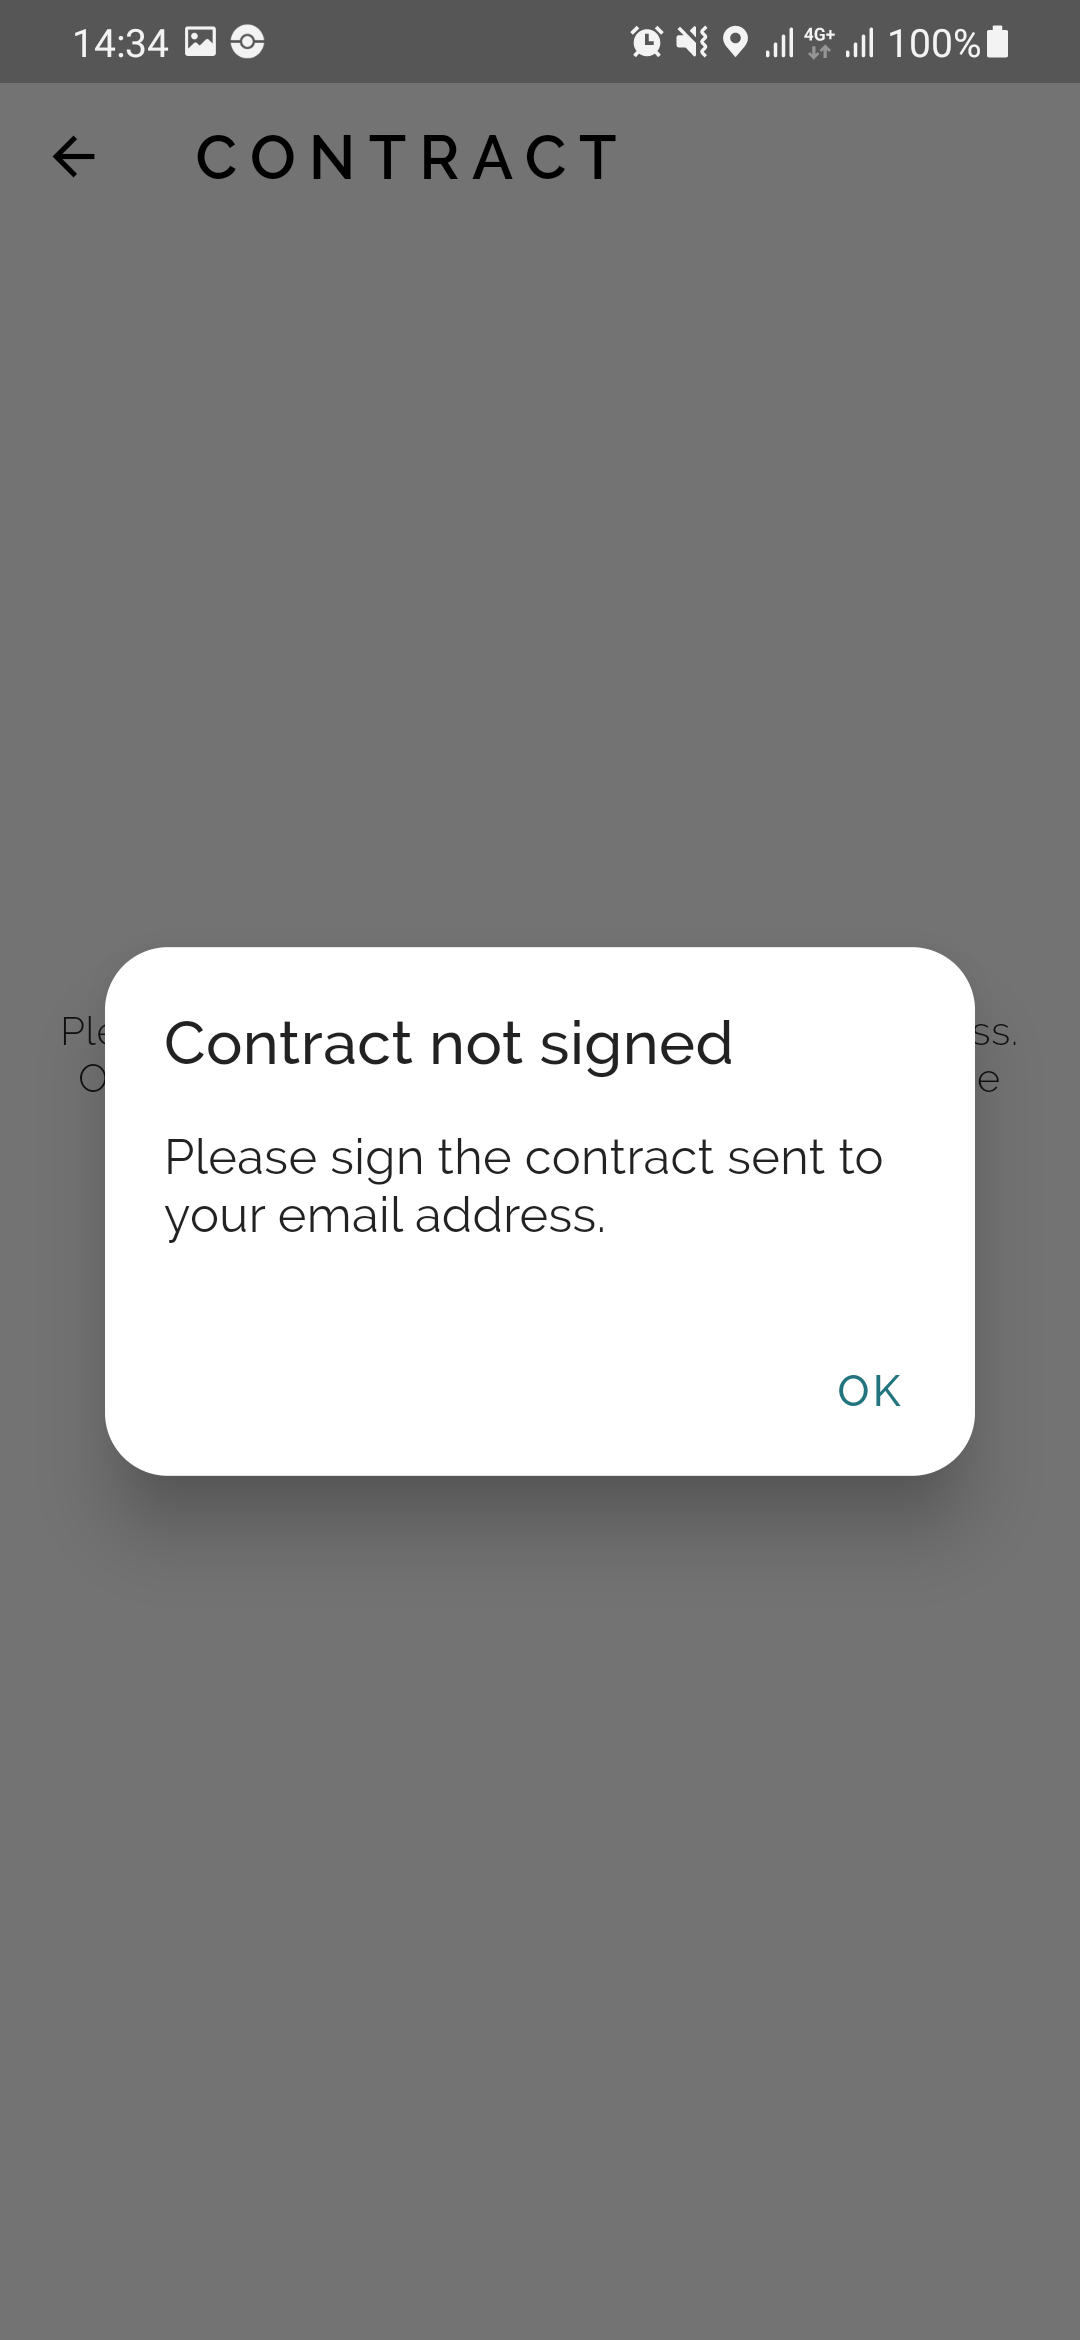
\includegraphics[height = 0.4\textheight]{ui_screenshots/app_screenshots/not_signed.png}
        \captionsetup{justification=centering}
        \caption{Vérification de signature avec un document non signé.}
        \label{fig:not_signed}
    \end{figure}
    \begin{figure}[H]
        \centering
        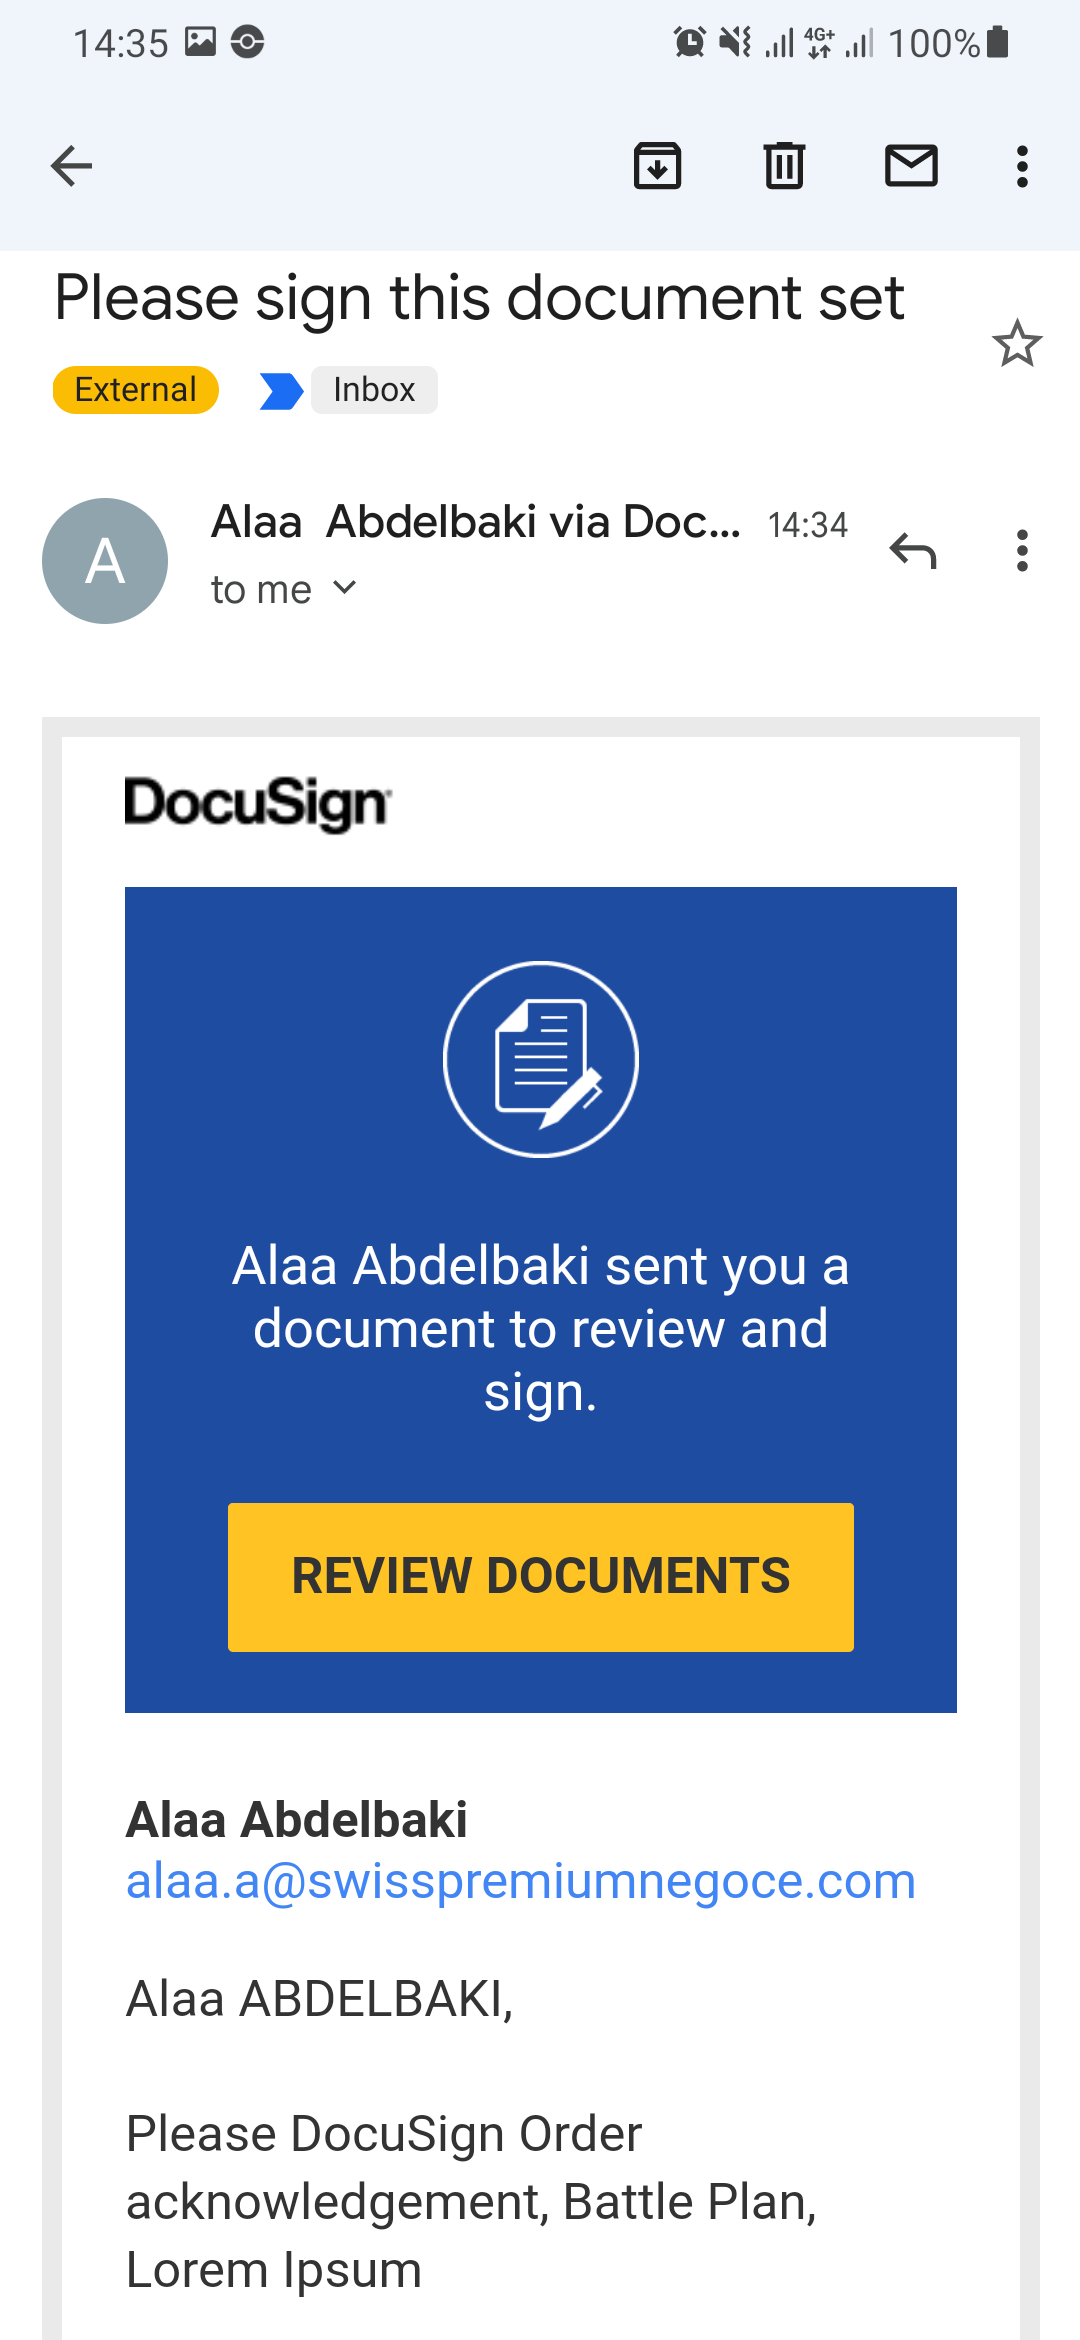
\includegraphics[height = 0.4\textheight]{ui_screenshots/app_screenshots/contract_email.png}
        \captionsetup{justification=centering}
        \caption{Email contenant les documents à signer.}
        \label{fig:sign_documents}
    \end{figure}
\end{multicols}
\vspace{1cm}
\begin{multicols}{2}
    \begin{figure}[H]
        \centering
        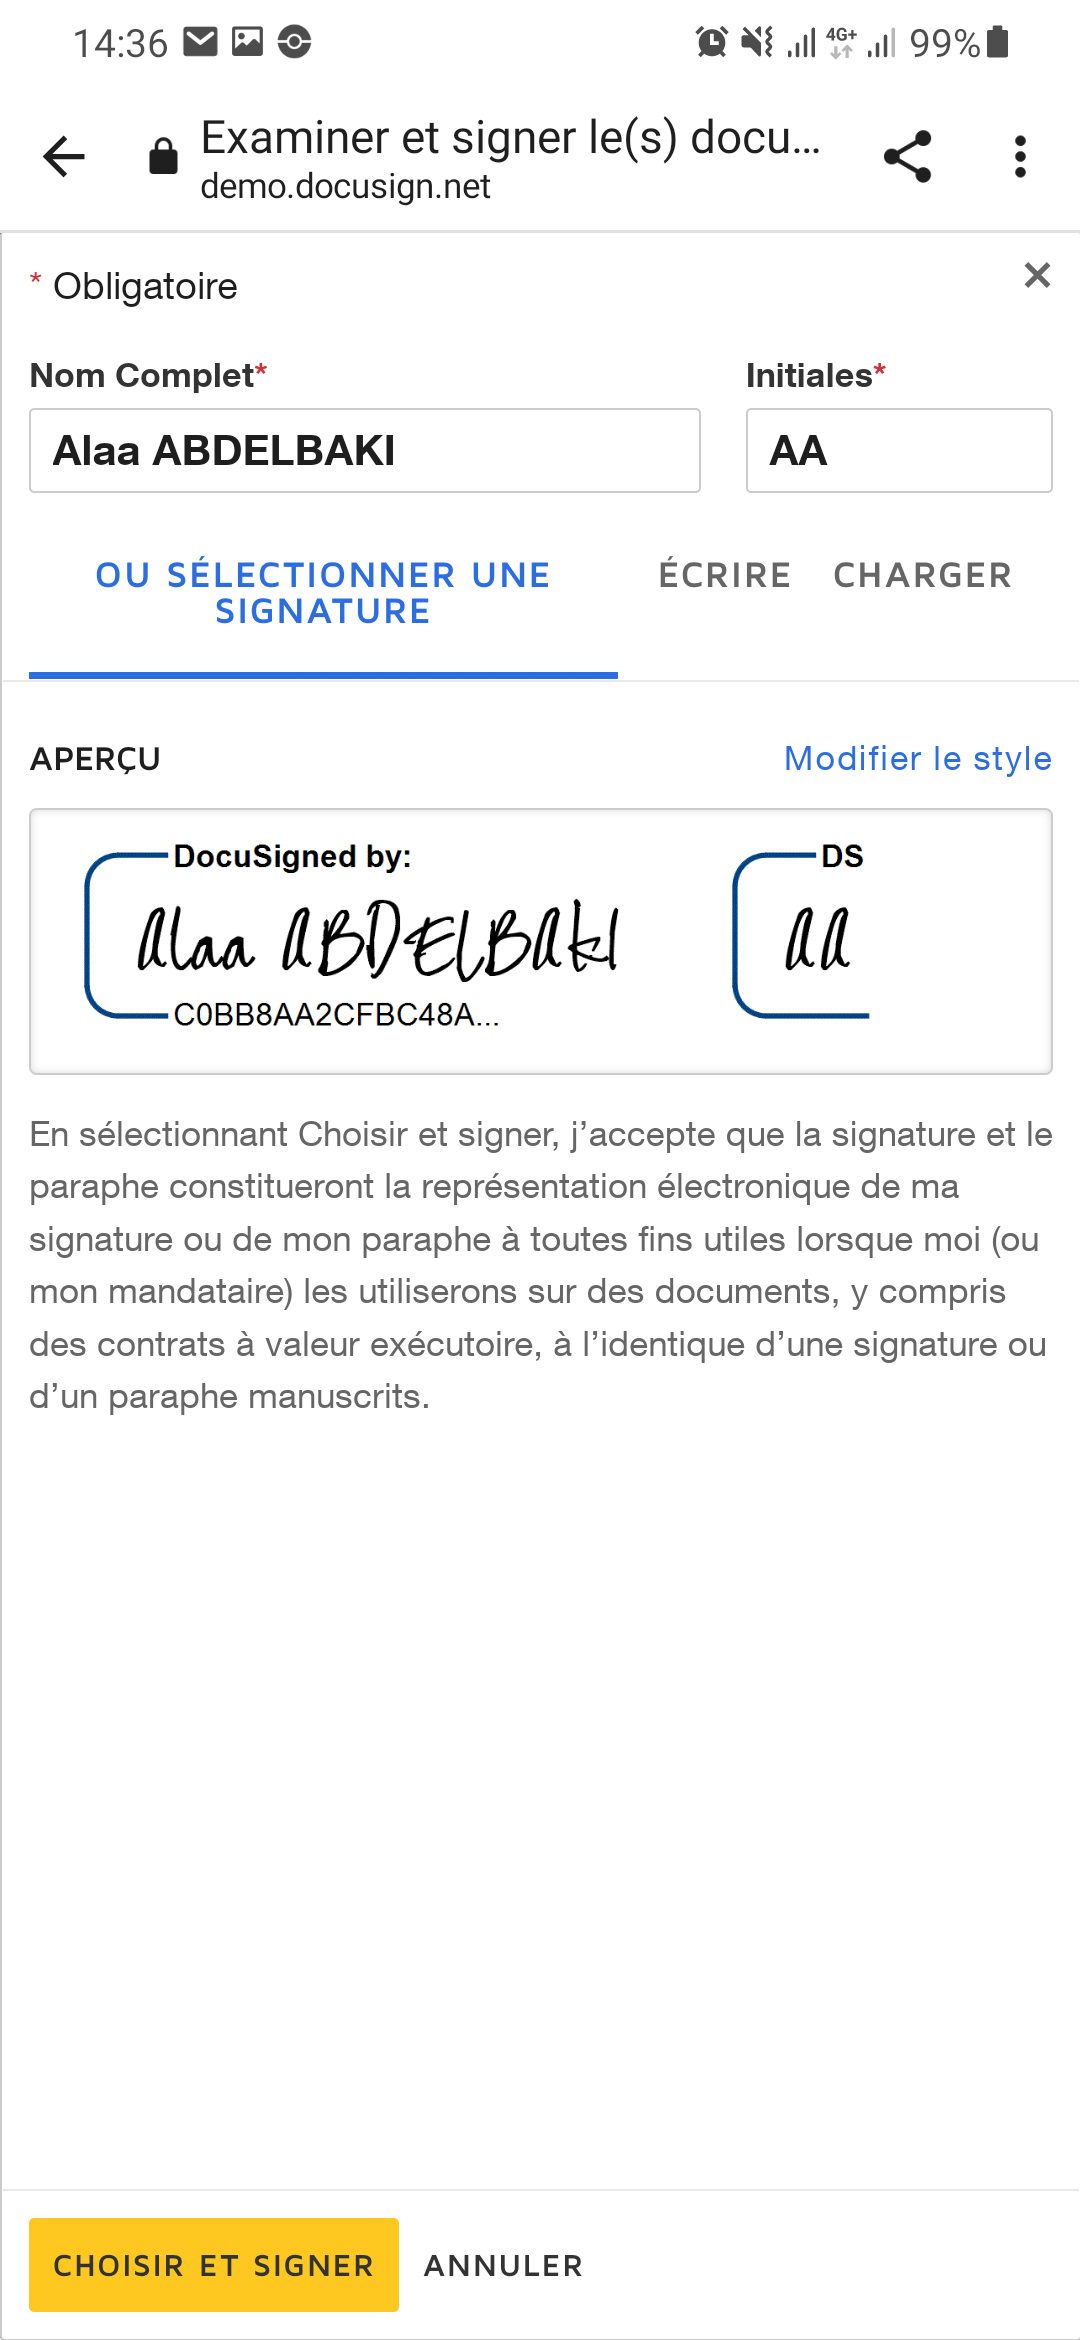
\includegraphics[height = 0.4\textheight]{ui_screenshots/app_screenshots/signature.png}
        \captionsetup{justification=centering}
        \caption{Choix de signature.}
        \label{fig:signature_select}
    \end{figure}
    \begin{figure}[H]
        \centering
        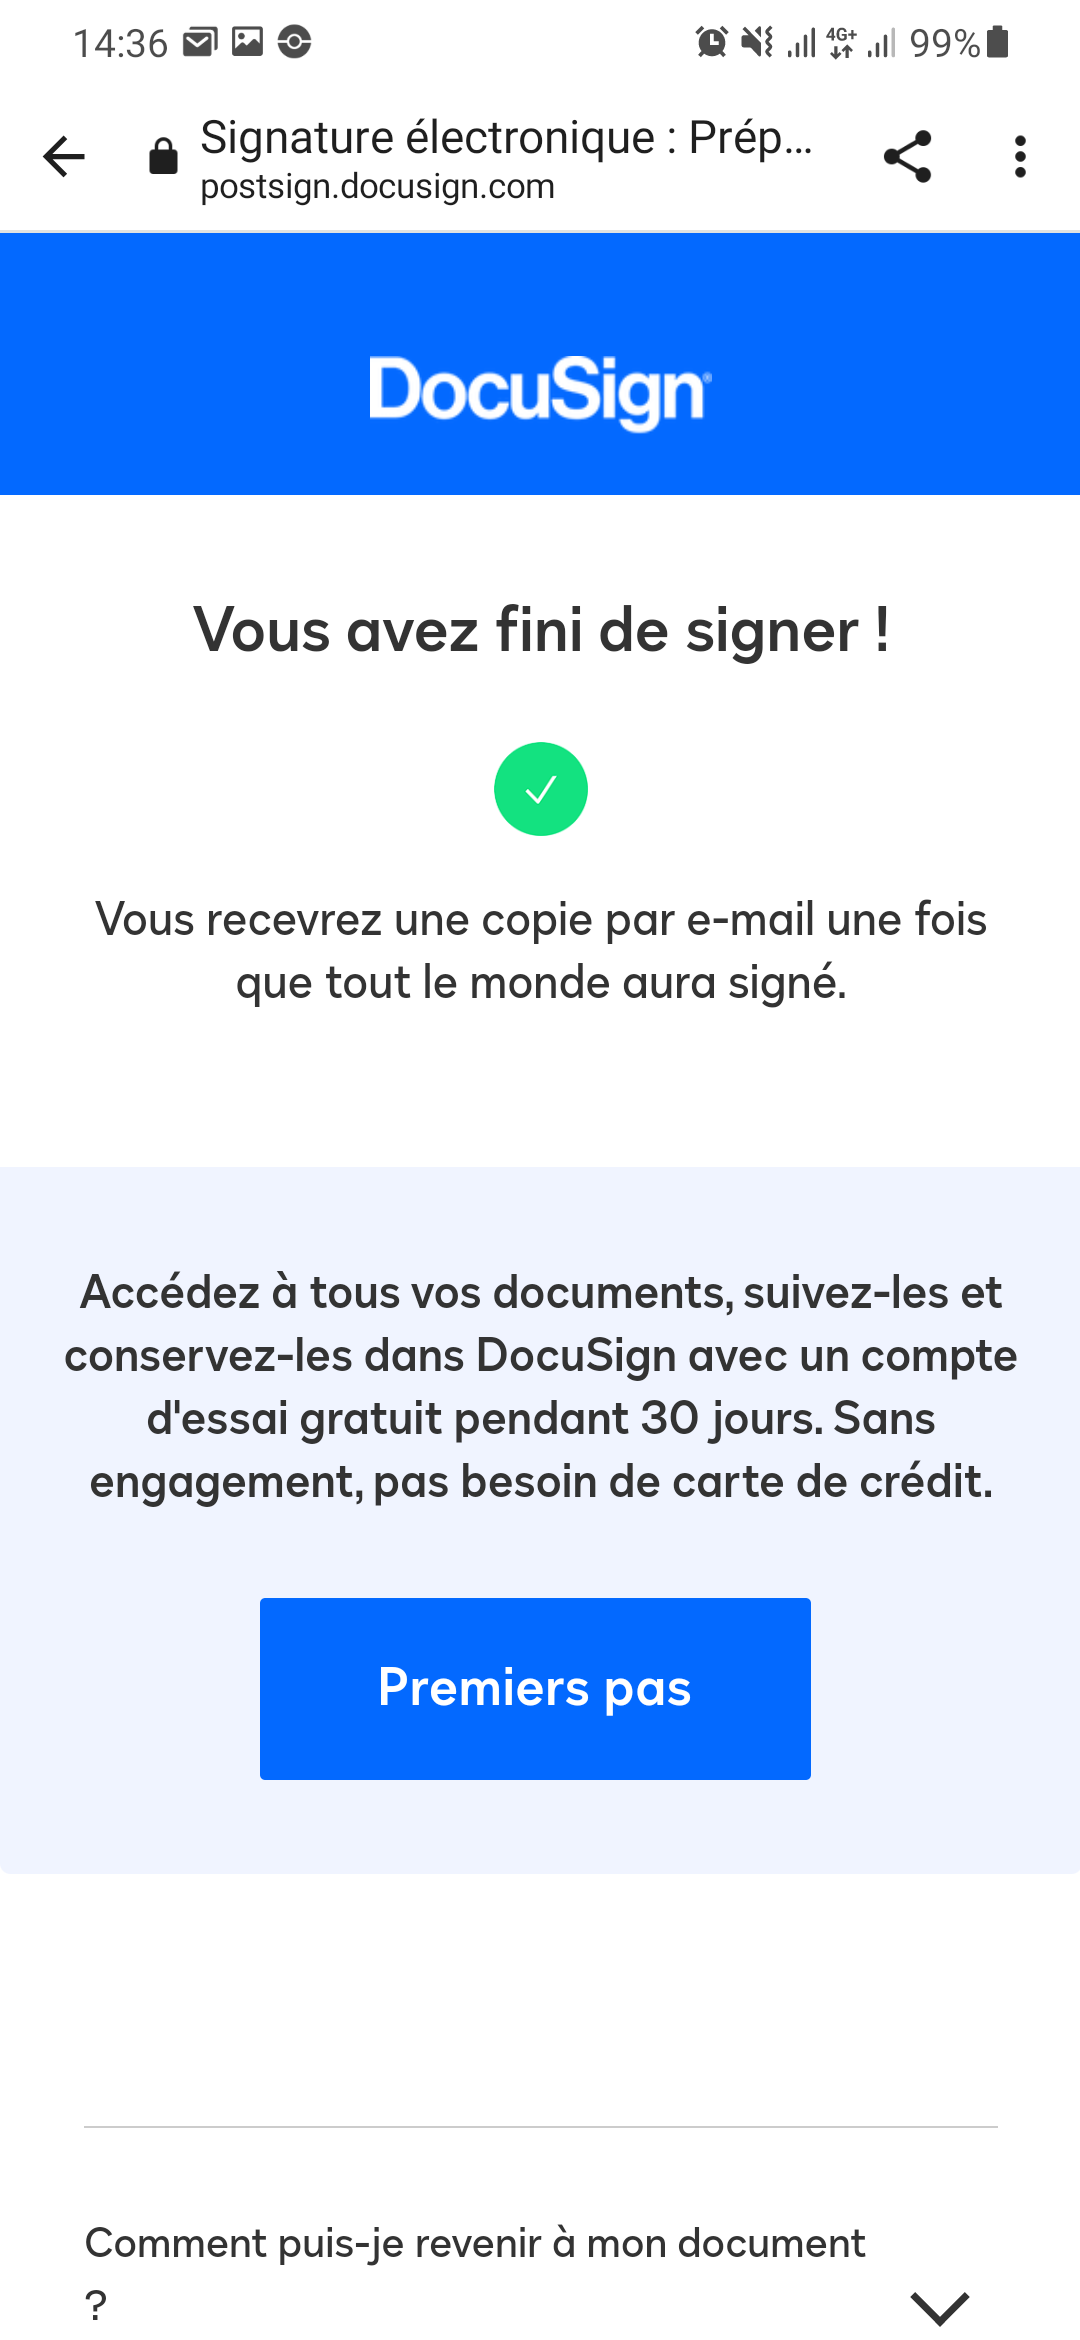
\includegraphics[height = 0.4\textheight]{ui_screenshots/app_screenshots/signature_end.png}
        \captionsetup{justification=centering}
        \caption{confirmation de signature.}
        \label{fig:confirm_sig}
    \end{figure}
\end{multicols}
\section{Paiement}
Pour le paiement des services offerts par SPN Cars, l'utilisateur utilisera <<Apple Pay>> s'il utilise un iPhone ou <<Google Pay>> s'il utilise un smartphone Android, qui sont, grâce à leurs haute disponibilités, le choix optimal pour effectuer des paiements en ligne avec son propre smartphone.\\
Pour effectuer un paiement avec l'application SPN Cars, il suffit de signer le contrat de location dans le cas de location de voitures, ou sélectionner une voiture dans le cas de demande de transfert, après la page de paiement avec le bouton de paiement selon le type de smartphone sera affiché. Lors de l'appui, L'interface des applications de paiement adéquates sera affichée pour continuer la transaction. Une fois terminé, l'utilisateur sera redirigé vers la page d'accueil si le paiement est effectué, ou un message d'erreur sera affiché si non.
\vspace{1cm}

\begin{multicols}{2}
    \begin{figure}[H]
        \centering
        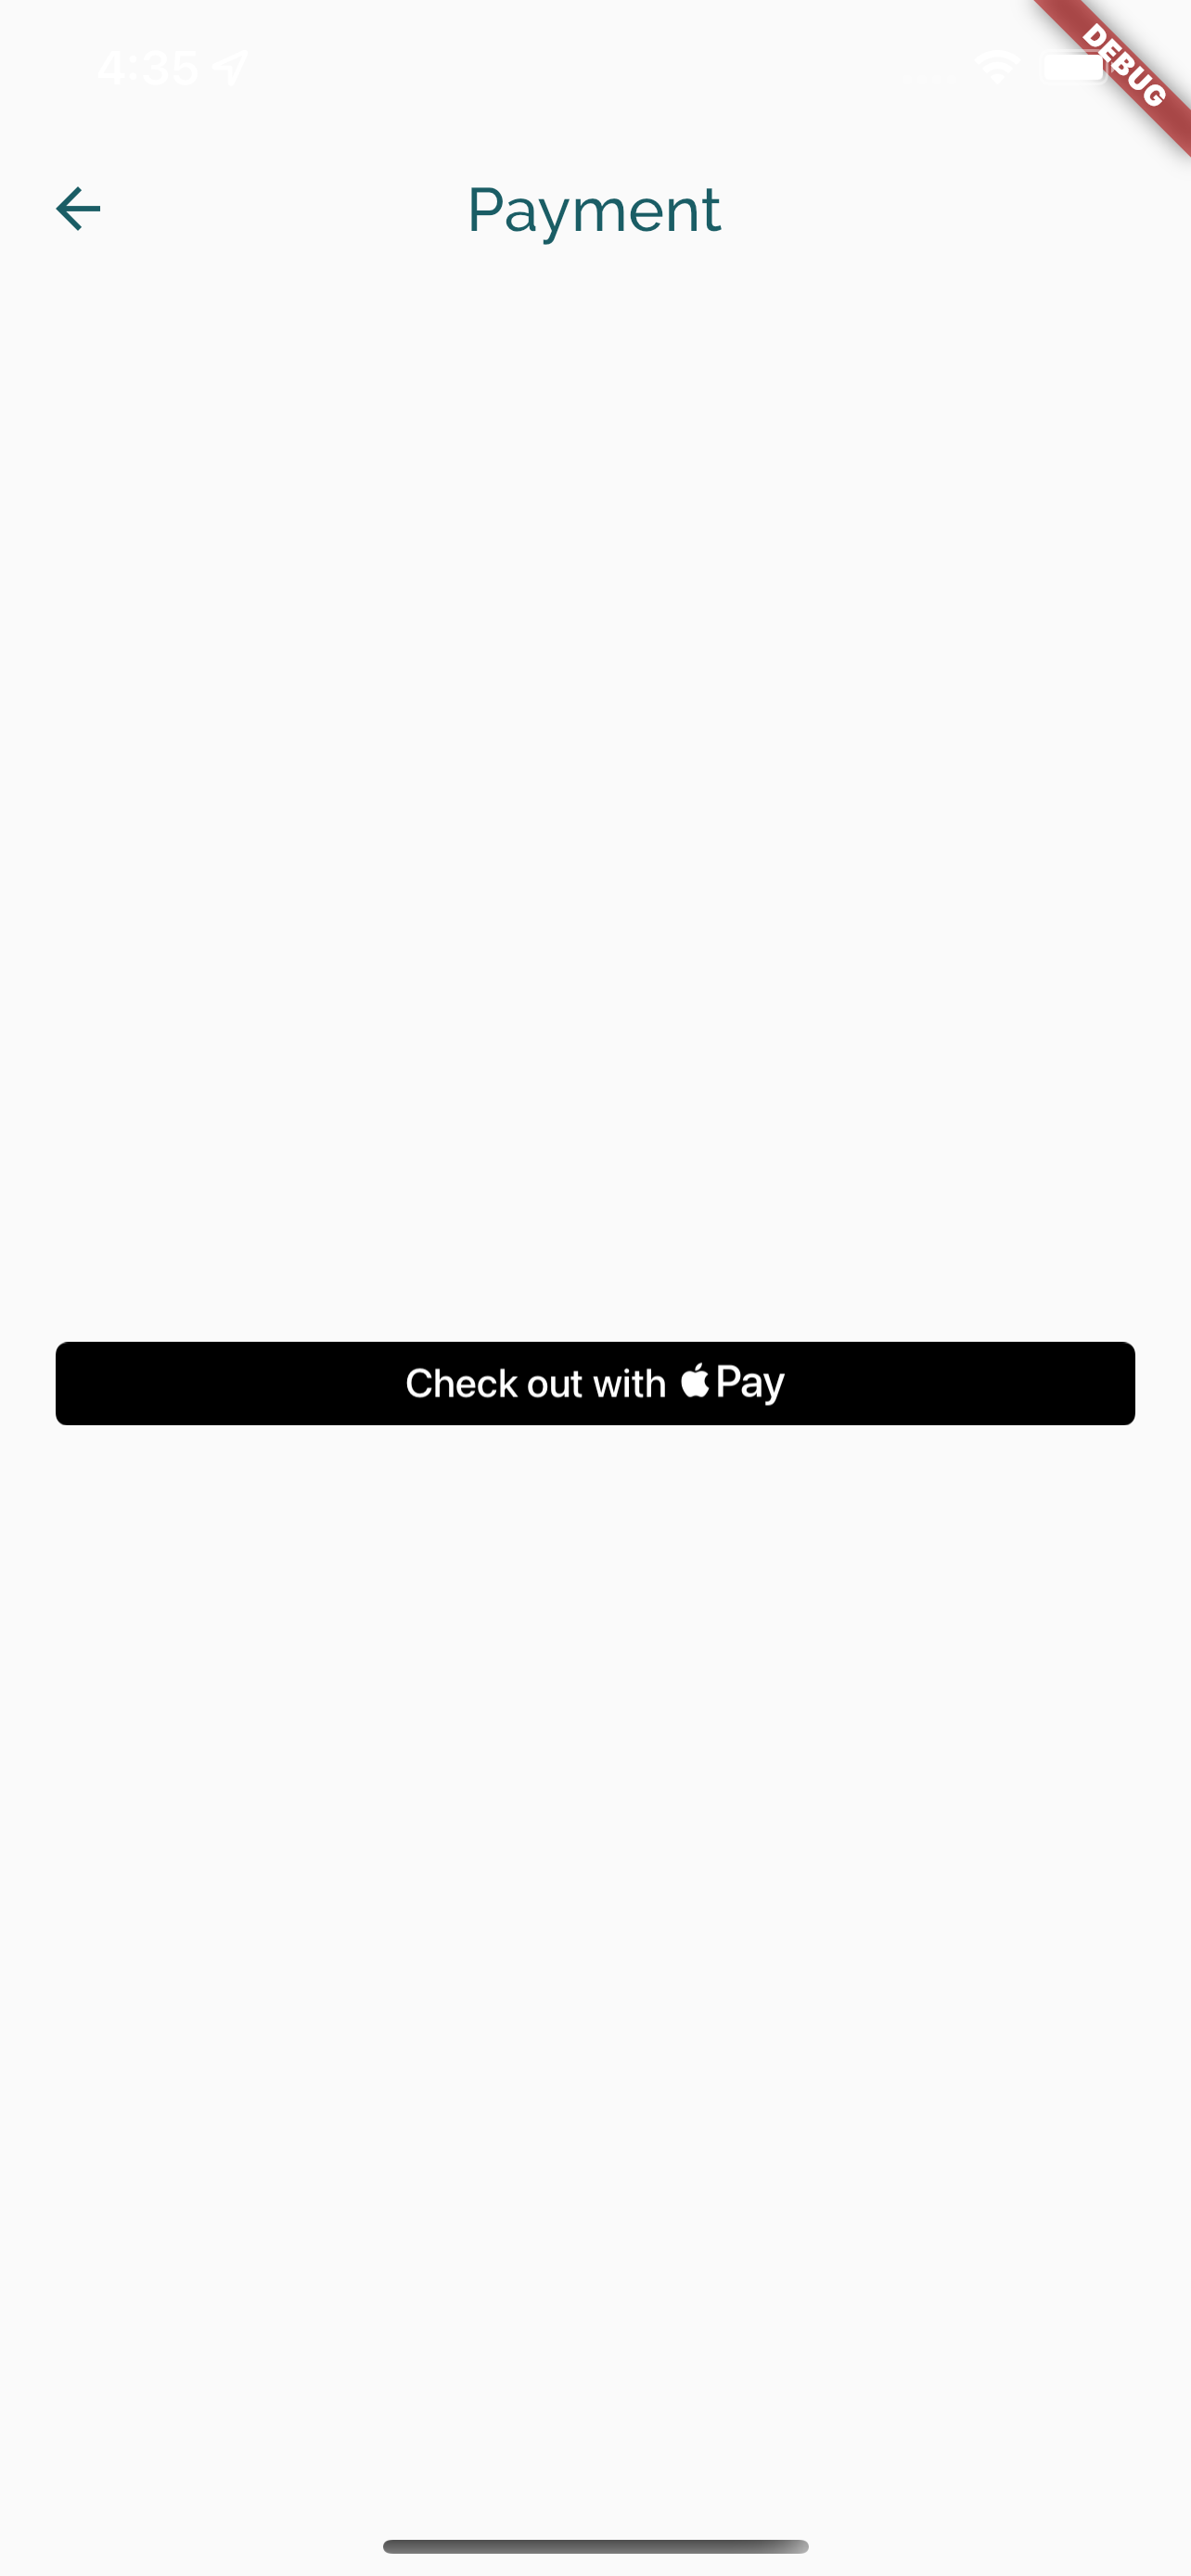
\includegraphics[height = 0.4\textheight]{ui_screenshots/app_screenshots/checkout.png}
        \captionsetup{justification=centering}
        \caption{Interface de paiement.}
        \label{fig:checkout}
    \end{figure}
    \begin{figure}[H]
        \centering
        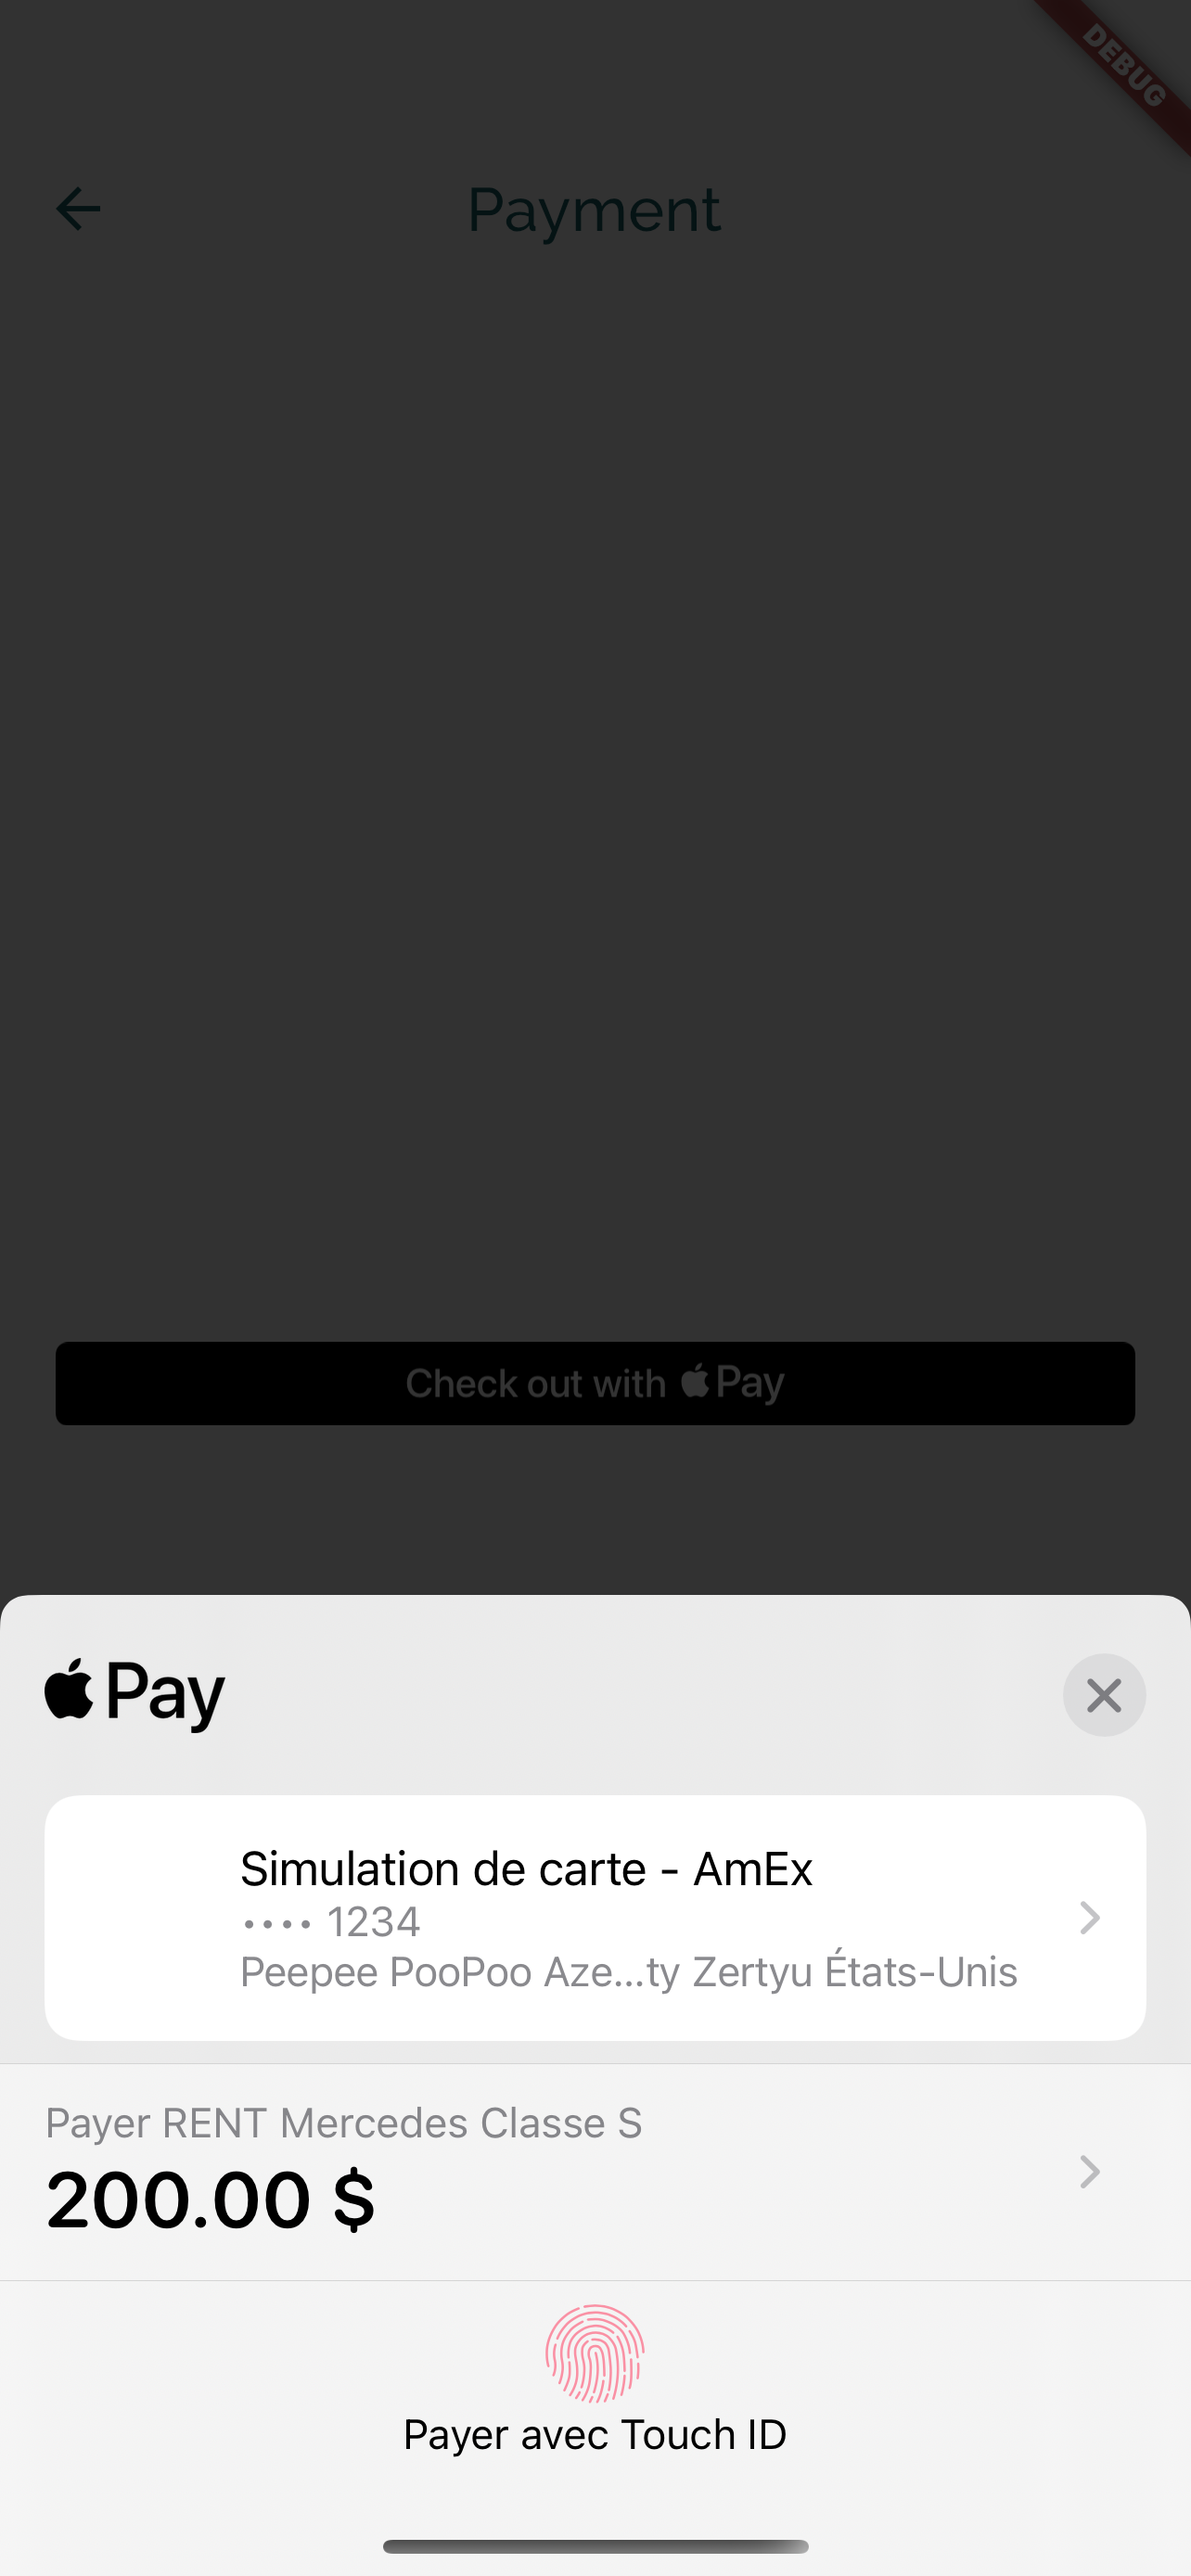
\includegraphics[height = 0.4\textheight]{ui_screenshots/app_screenshots/pay_details.png}
        \captionsetup{justification=centering}
        \caption{Détails de paiement.}
        \label{fig:pay_details}
    \end{figure}
\end{multicols}
\section{Localiser une voiture}
Lorsqu'une réservation atteint la date de début et sera affichée dans la page d'accueil, le client peut appuyer sur la réservation et voir plus de détails sur sa réservation et sa voiture. Une fois appuyé sur le bouton <<See more>>, le client sera redériger vers une page qui affiche la position de sa voiture sur un plan. Cette position sera mise à jour en temps réel si le chauffeur est en train de conduire la voiture.\\
\noindent La page permet aussi d'afficher les informations basiques du chauffeur avec une possibilité de le contacter soit par appel téléphonique soit par message.
\begin{figure}[H]
    \centering
    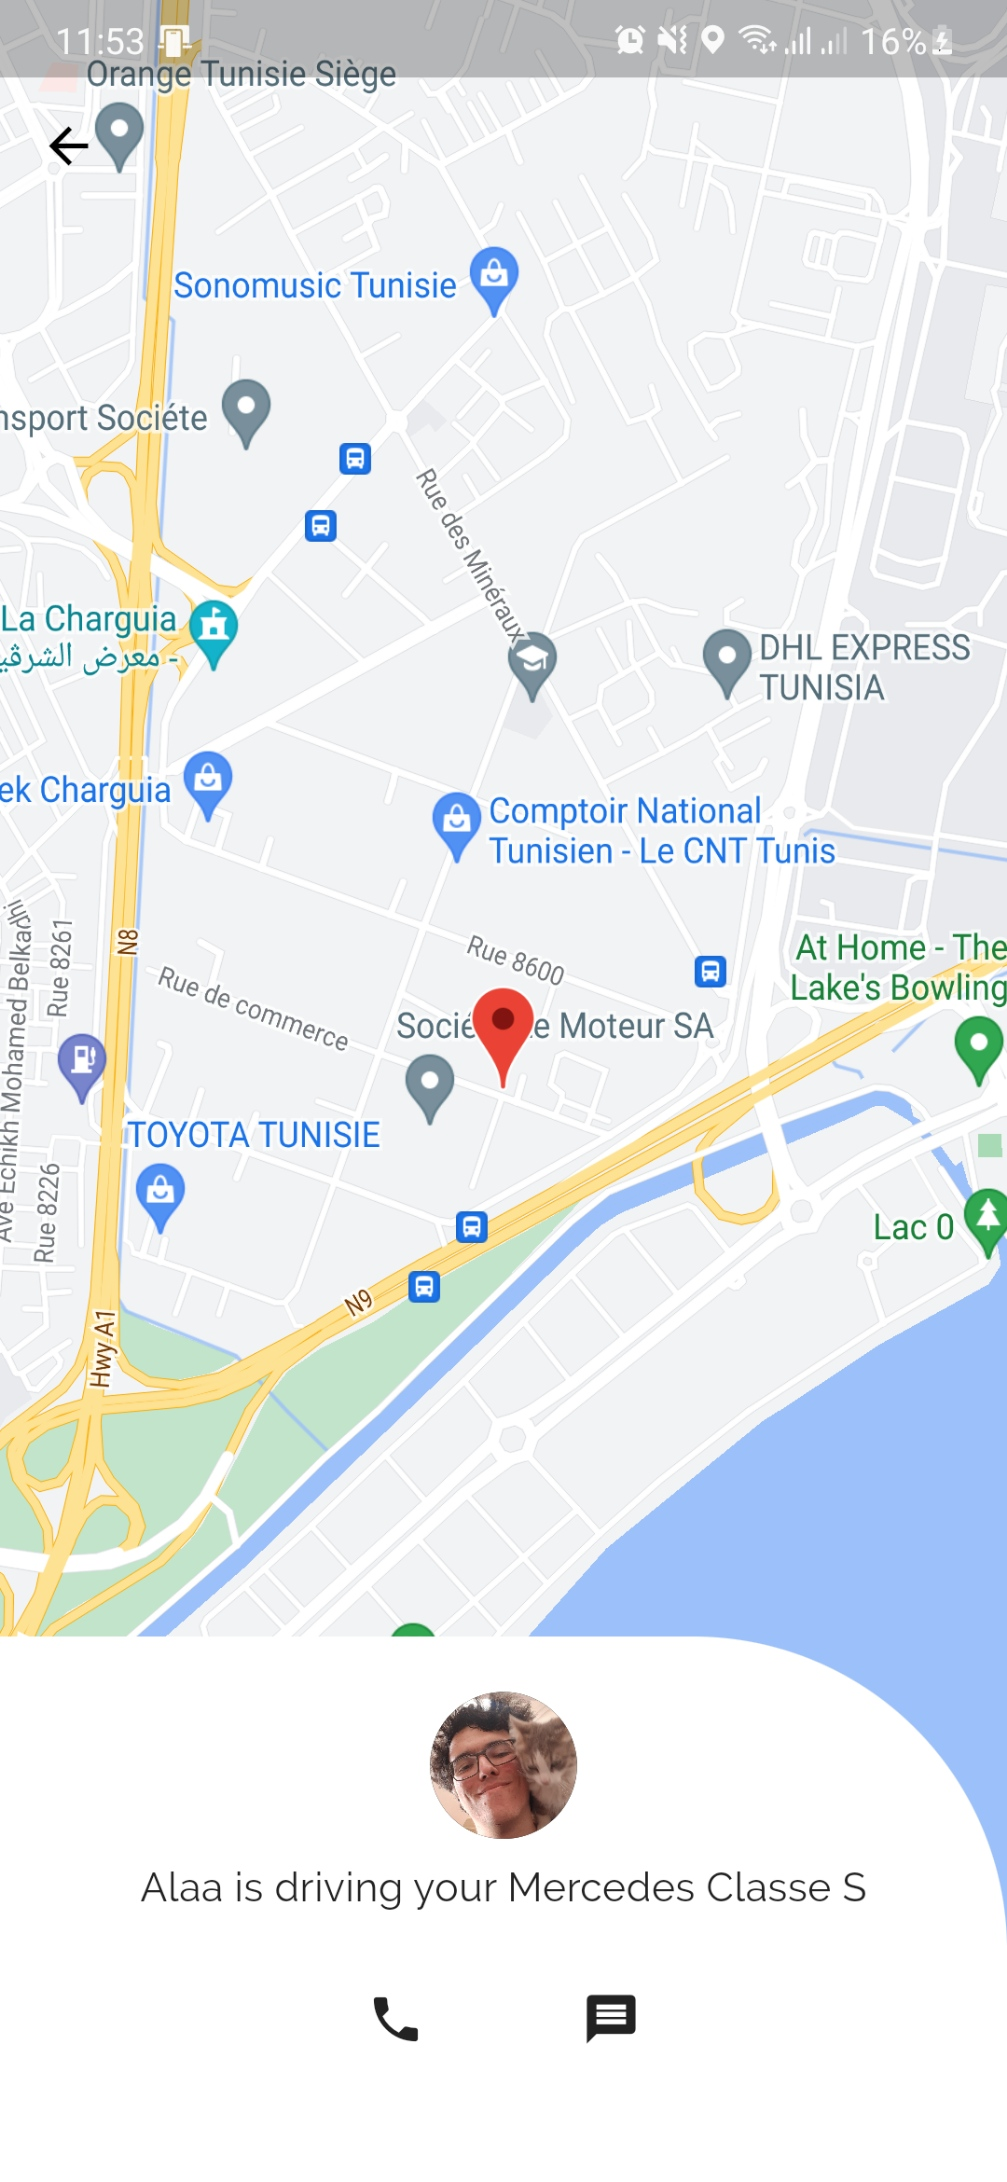
\includegraphics[height= 0.4\textheight]{ui_screenshots/app_screenshots/details.png}
    \captionsetup{justification=centering}
    \caption{Affichage des détails de la réservation.}
    \label{fig:res_details}
\end{figure}
\section{Messagerie instantanée}
Une fois que l'utilisateur a appuyé sur le bouton pour contacter le chauffeur par messagerie instantanée, l'utilisateur est redirigé vers une page de messagerie avec le chauffeur où ils peuvent échanger des messages.\\
\noindent L'utilisateur peut aussi retourner vers sa liste de conversations et afficher ses anciens messages depuis la page d'accueil.
\clearpage
\begin{multicols}{2}
    \begin{figure}[H]
        \centering
        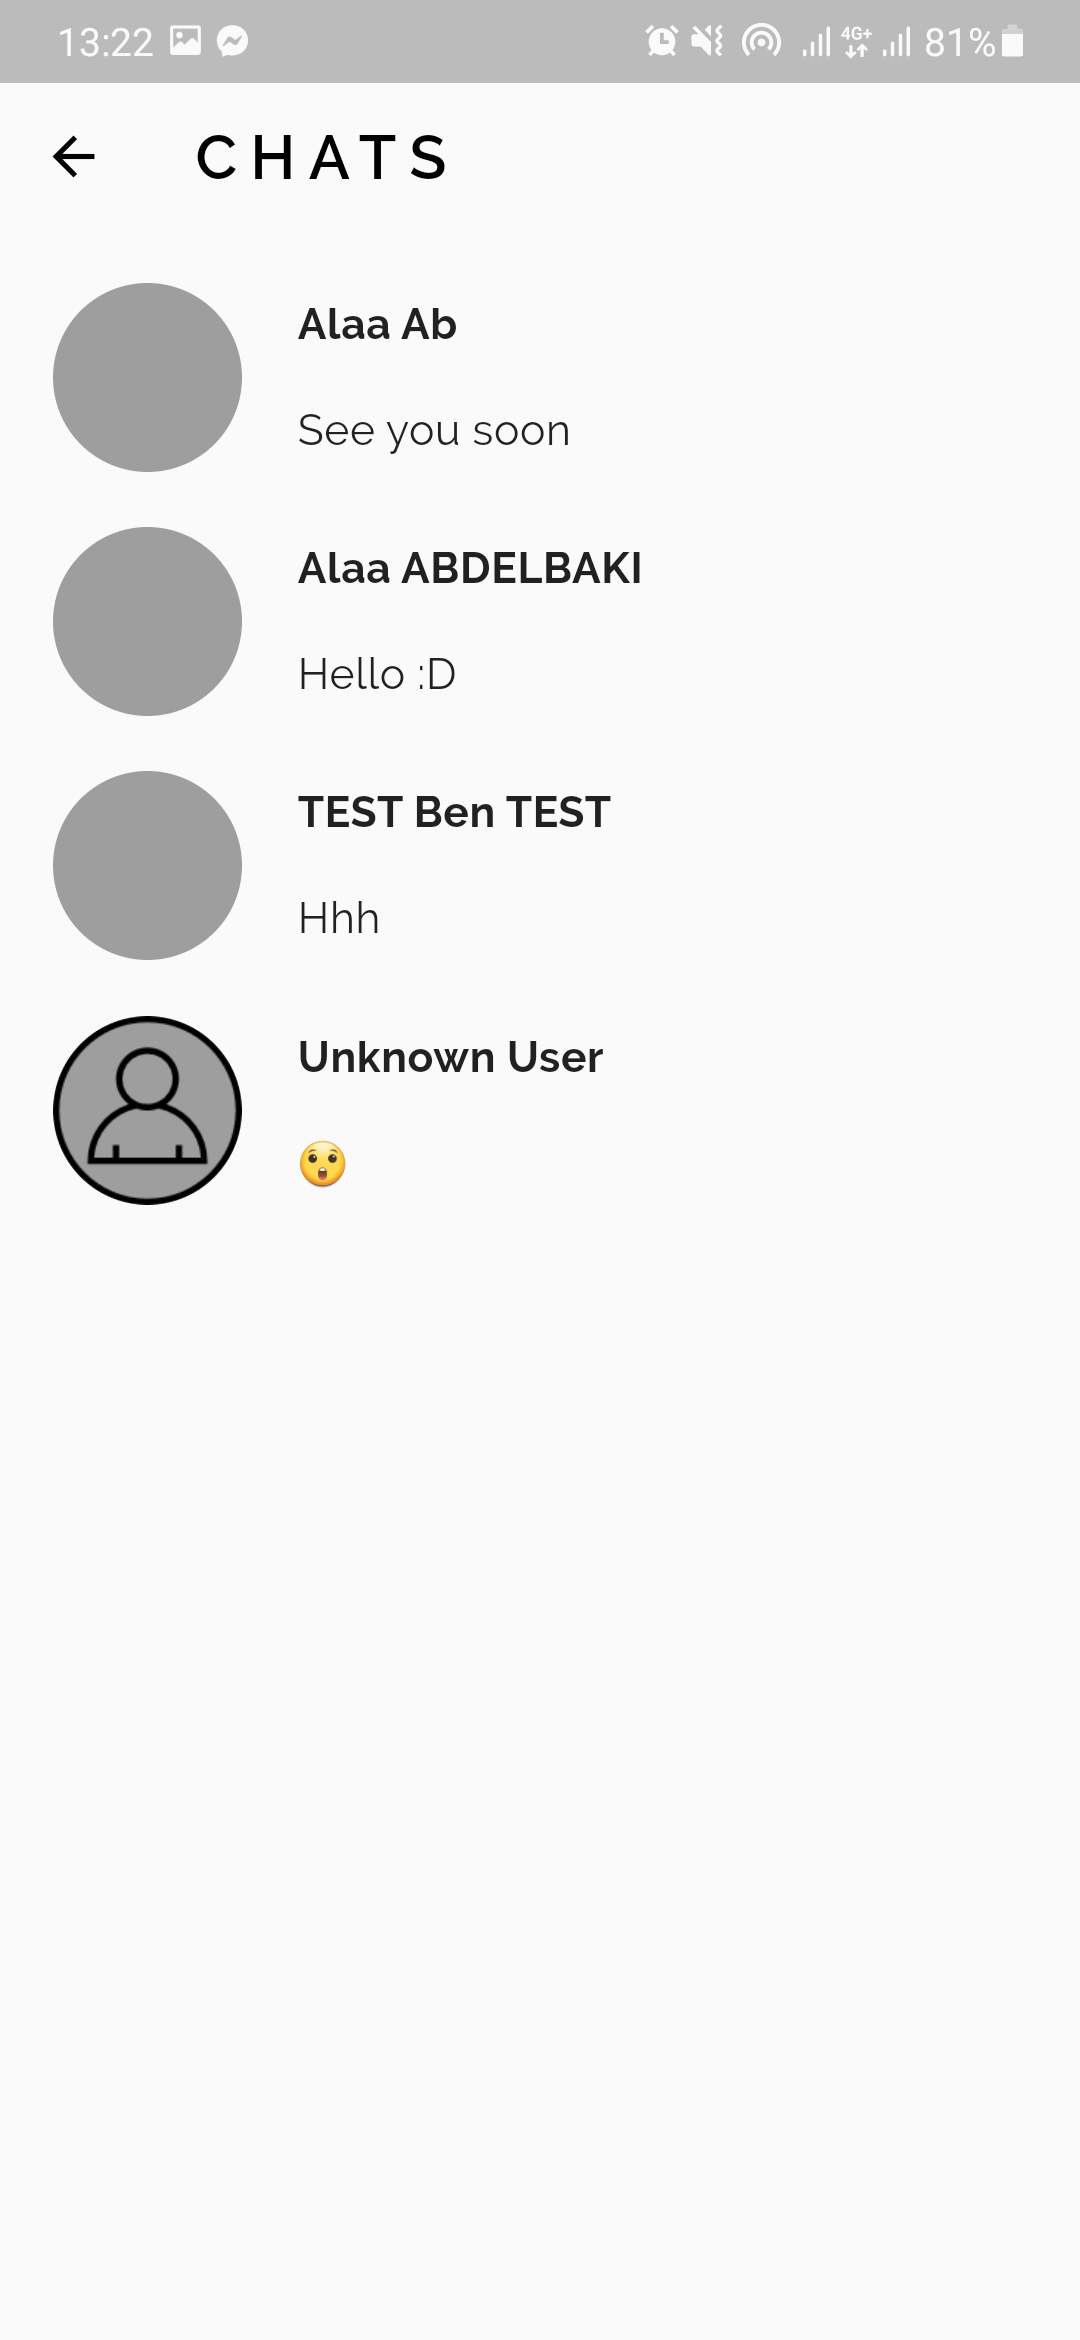
\includegraphics[height = 0.4\textheight]{ui_screenshots/app_screenshots/messages_list.png}
        \vspace{1cm}
        \captionsetup{justification=centering}
        \caption{Liste de messages de l'utilisateur.}
        \label{fig:message_list}
    \end{figure}
    \begin{figure}[H]
        \centering
        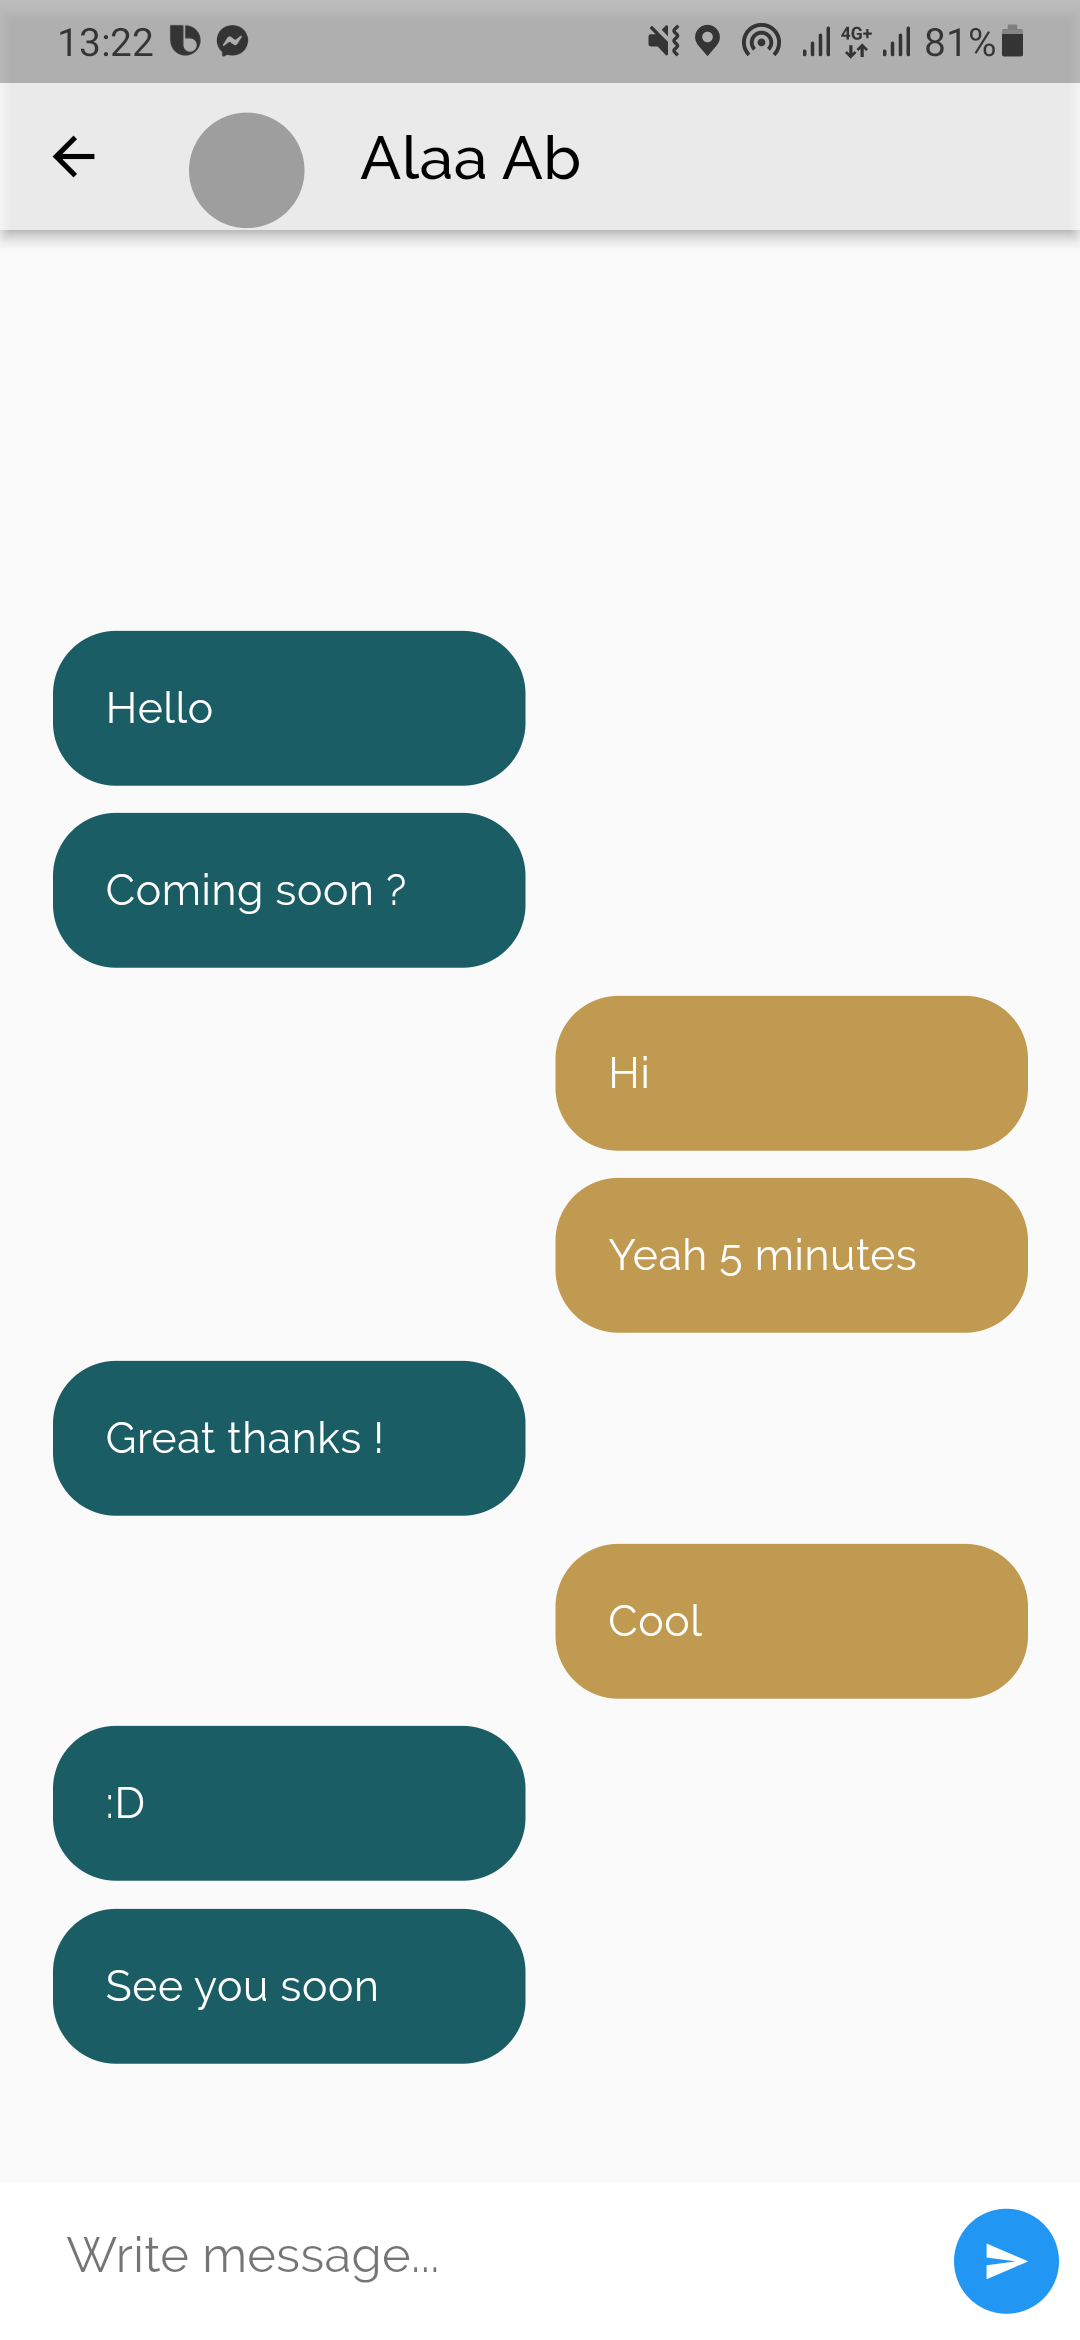
\includegraphics[height = 0.4\textheight]{ui_screenshots/app_screenshots/messages_details.png}
        \vspace{1cm}
        \captionsetup{justification=centering}
        \caption{Conversation avec l'utilisateur.}
        \label{fig:conversation}
    \end{figure}
\end{multicols}
\section{Documentation des API}
La documentation des APIs est une étape nécessaire dans le développement de n'importe quelle application. Une documentation accessible et facilement exploitable est une condition préalable au développement des API. Il est important d'avoir une documentation toujours à jour quand le code/les fonctionnalités de l'API évoluent.\\
\noindent Et puisque le modèle de développement chez SPN est centré sur le travail collaboratif, il est très important d'avoir une documentation claire et et facile à exploiter des APIs.

On va prendre un exemple de documentation de l'API de l'entitée <<Voiture>> où on a suivi les spécifications de Open Api pour créer la documentation de ses APIs.
\begin{figure}[H]
    \centering
    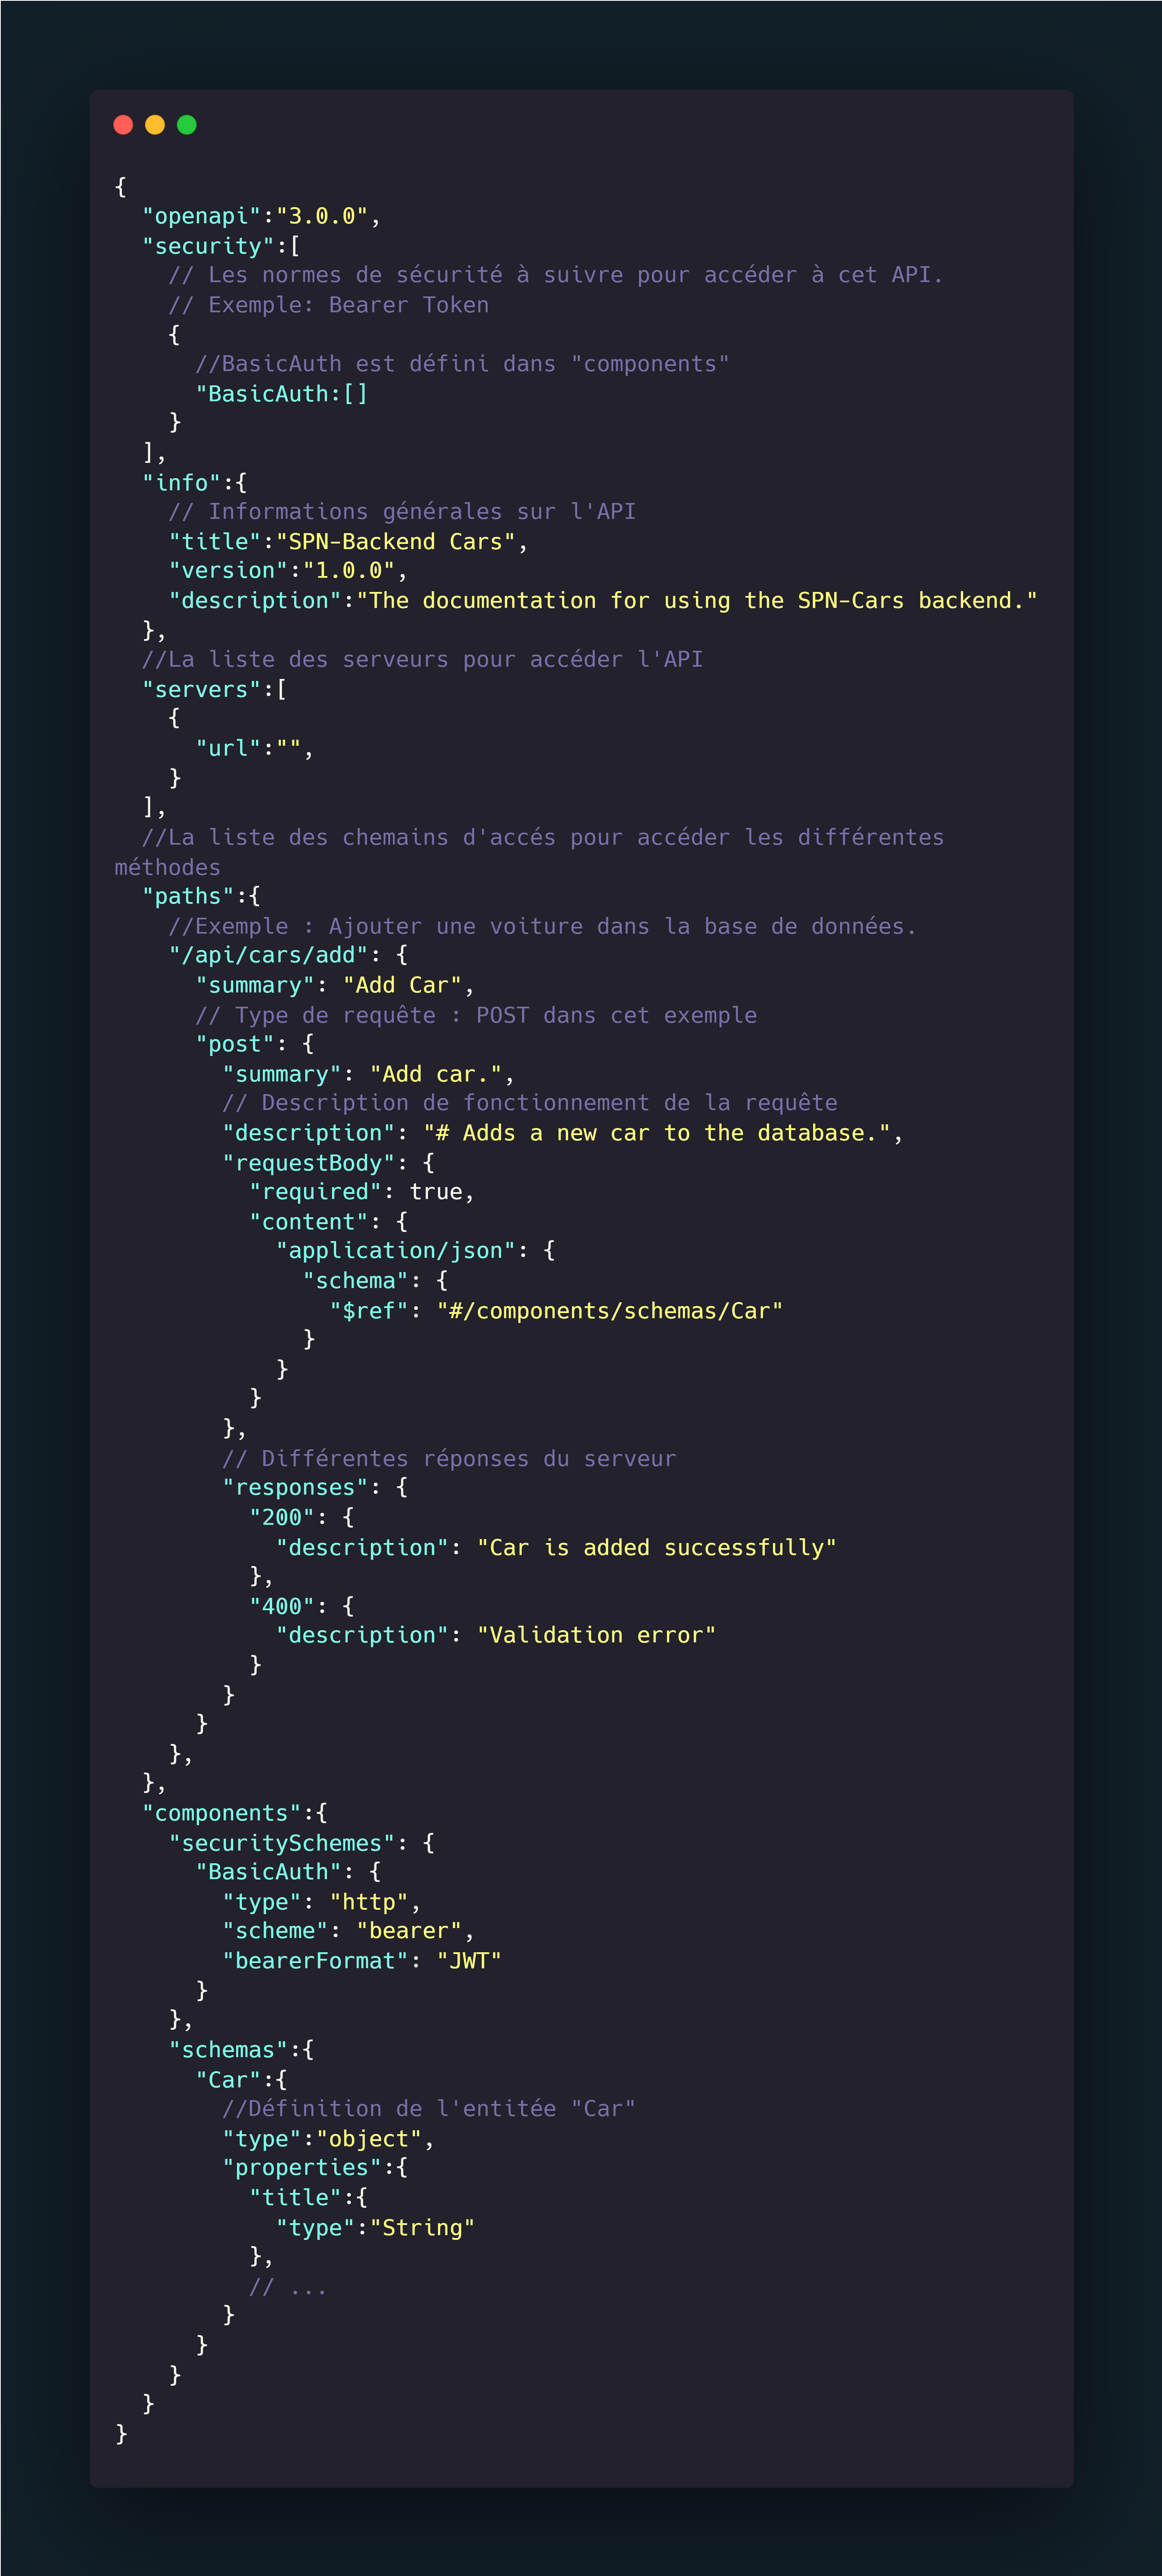
\includegraphics[height= \textheight]{openapi.png}
    \captionsetup{justification=centering}
    \caption{Schéma de documentation des API.}
    \label{fig:api_doc_schema}
\end{figure}
\newpage
\begin{figure}[H]
    \centering
    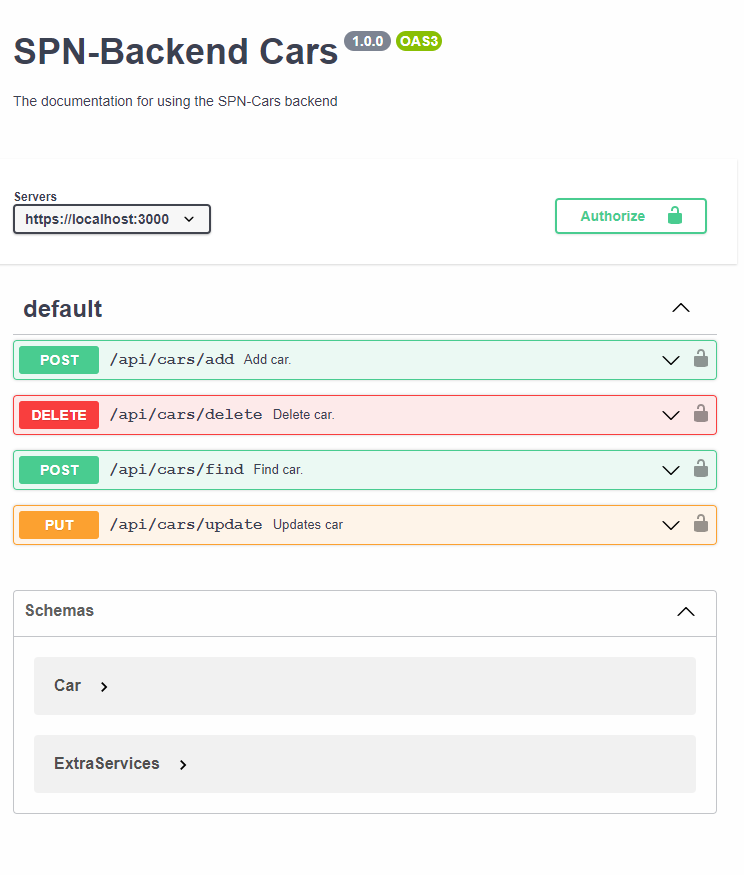
\includegraphics[height= 0.8\textheight,width=\textwidth]{api.png}
    \captionsetup{justification=centering}
    \caption{Documentation des API.}
    \label{fig:api_doc}
\end{figure}
\begin{figure}[H]
    \centering
    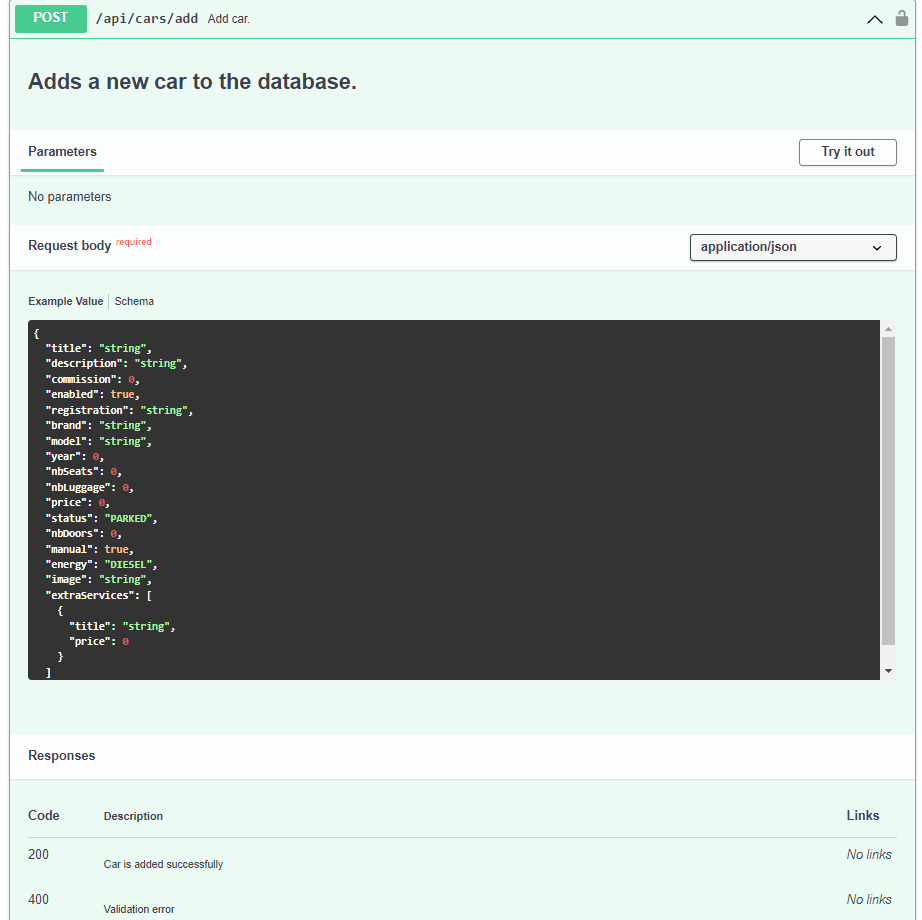
\includegraphics[height= 0.8\textheight,width=\textwidth]{add_car.png}
    \captionsetup{justification=centering}
    \caption{Détails API ajout voiture.}
    \label{fig:api_doc_detail}
\end{figure}
\clearpage
\section{Conclusion}
Dans ce chapitre on a présenté la réalisation de l'application, où on a décrit chaque fonctionnalité de l'application avec des captures d'écran qui montrent les différentes interfaces. On a commencé par l'étape de création de compte et connexion qui permettra au client d'utiliser les différents services offerts par l'application et on a passé par les différentes fonctionnalités une par une.\\
\noindent On a présenté aussi l'étape de documentation des APIs qui permettra de faciliter la collaboration avec d'autres équipes et l'amélioration de leur fonctionnement dans le futur.